\chapter{Analysis of the characteristics}\label{ana_char}
In this chapter, we will analyse and measure different characteristics from various Neural Network architectures with the purpose of finding useful correlations which we can use in a later stage. In order to achieve this goal, we will use our understanding from chapter \ref{char_nn} of each metric of Neural Network and the tool we developed in section \ref{sec:my_bench}. \\
In challenges such as the ImageNet classification challenge (\cite{ILSVRC15}) the ultimate goal is to achieve the highest accuracy possible, neglecting other performance metrics like inference time. \cite{DBLP:journals/corr/CanzianiPC16}\\
Although accuracy is of high importance, in practical applications other metrics are to be considered as well, depending on the different requirements. As pointed out by \textit{Canziani et al.} in \cite{DBLP:journals/corr/CanzianiPC16}, metrics like inference time, parameters and operations count are hard constraints
for the deployment of Neural Networks in practical applications. Furthermore, training time is often a time consuming process which highly depends on factors like the complexity of the task, size of the network and training set(\cite{118273}). \\
Finding relations between these metrics and other factors as well, like influence of a given input feature to the prediction of the model (\cite{hooker2019benchmark}), will allow us to optimise applications, saving time and resources in the process.
\section{Test Environment}
All the experiments have been run on the same machine running Ubuntu 20.04.3 LTS (Focal Fossa). For the specific of the machine, please refer to table \ref{tab:gpu_info}
\begin{table}[h]
\centering
\begin{tabular}{|l  |r|}
 \hline
CPU & AMD EPYC 7452 32-Core Processor\\
CPU MHz&                     1499.324\\
CPU max MHz&                     2350,0000\\
CPU min MHz&                     1500,0000\\
Total memory&       1056709772 kB\\
GPU&    Nvidia A100-PCIE-40GB\\
Number of GPUs & 8\\
\hline
\end{tabular}
\caption{Specifics of the machine which run the experiments}
\label{tab:gpu_info}
\end{table}

It is assumed for all the use cases that, if no specification is made, the training of the models has been carried out by the \textit{fit\_one\_cycle()} function present in fastai using the default learning rate. Furthermore, the models have not been pre-trained, hence no transferred learning is applied, and the models have been trained using full precision. \\







\section{Fist Experiment}
For this use case, we are going to use the dataset proposed by \textit{Giselsson et al.} in \cite{giselsson2017public}, which we are going to refer to as the ‘plant\_seedlings\_v2’ dataset. This dataset contains \textasciitilde 1000 RGB images with a resolution of 10 pixels per mm divided in 12 different plant species. The plants in the dataset are listed in table \ref{tab:dataset_species}. This dataset contains pictures of one of the most common weeds found in sugar beet plantations, a plant commonly referred to as ''charlock''. \cite{cioni_weed_2010}\\
Even though the dataset is mainly focused on seedlings and it contains pictures of other plants as well, this will give us proper insights of the models’ behaviours in a farming setting.
\begin{table}[ht]
\centering
\begin{tabular}{|c|c|c|}
\hline
    English & Latin \\
\hline
    Maize & Zea mays L.\\
    Common wheat & Tricicum aestivum L.\\
    Sugar beet & Beta vulgaris var. altissima\\
    Scentless Mayweed & Matricaria perforata Mérat\\
    Common Chickweed & Stellaria media\\
    Shepherd’s Purse & Capsella bursa-pastoris\\
    Cleavers& Galium aparine L.\\
    Redshank& Polygonum persicaria L.\\
    Charlock& Sinapis arvensis L.\\
    Fat Hen& Chenopodium album L.\\
    Small-flowered Cranesbill & Geranium pusillum\\
    Field Pansy& Viola arvensis\\
    Black-grass& Alopecurus myosuroides\\
    Loose Silky-bent& Apera spica-venti\\
    \hline
\end{tabular}
\caption[Categories of the ‘plant\_seedlings\_v2’ dataset]{Categories of the ‘plant\_seedlings\_v2’ dataset \cite{giselsson2017public} }
\label{tab:dataset_species}
\end{table}

The first metrics we are going to analyse are training time, number of epochs and accuracy. We will study those metrics in order to recognize some patterns and use those to be able to find correlations between the three, with the final aim being able to predict one of them, whilst knowing the others. These prediction patterns can be used to save time during the learning process in future applications, as we can estimate the accuracy before starting the process.  \\
The tool ran the test three times for 50, 100 and 200 epochs. 
We are going to start our analysis by studying the results obtained when trained for 100 epochs, which are shown in Fig. \ref{fig:seedlings_100_epoch_accuracy} and \ref{fig:seedlings_100_acc}. \\
Alexnet is the model that achieved the lowest accuracy, overall reaching \textasciitilde86\% after 99 epochs. The highest accuracy has been achieved by Resnet101, peaking at \textasciitilde97\% after 66 epochs. Moreover, VGG16 and VGG19 achieved the same peak accuracy at \textasciitilde95\%, however VGG16 required 13 epochs less (43 compared to the 56 needed for VGG19). Similarly, Resnet18 and Resnet34 achieved comparable top accuracies at  94.39\% and 94.48\% respectively, however Resnet34 required considerably less time to reach this number peaking after 62 epochs, while Resnet18 achieved this number when the training cycle was almost done, namely after 96 epochs. An overview of the performances of all the models can be seen in table \ref{tab:performances_seeds}. 

\begin{figure}[h]
       \centering 
	    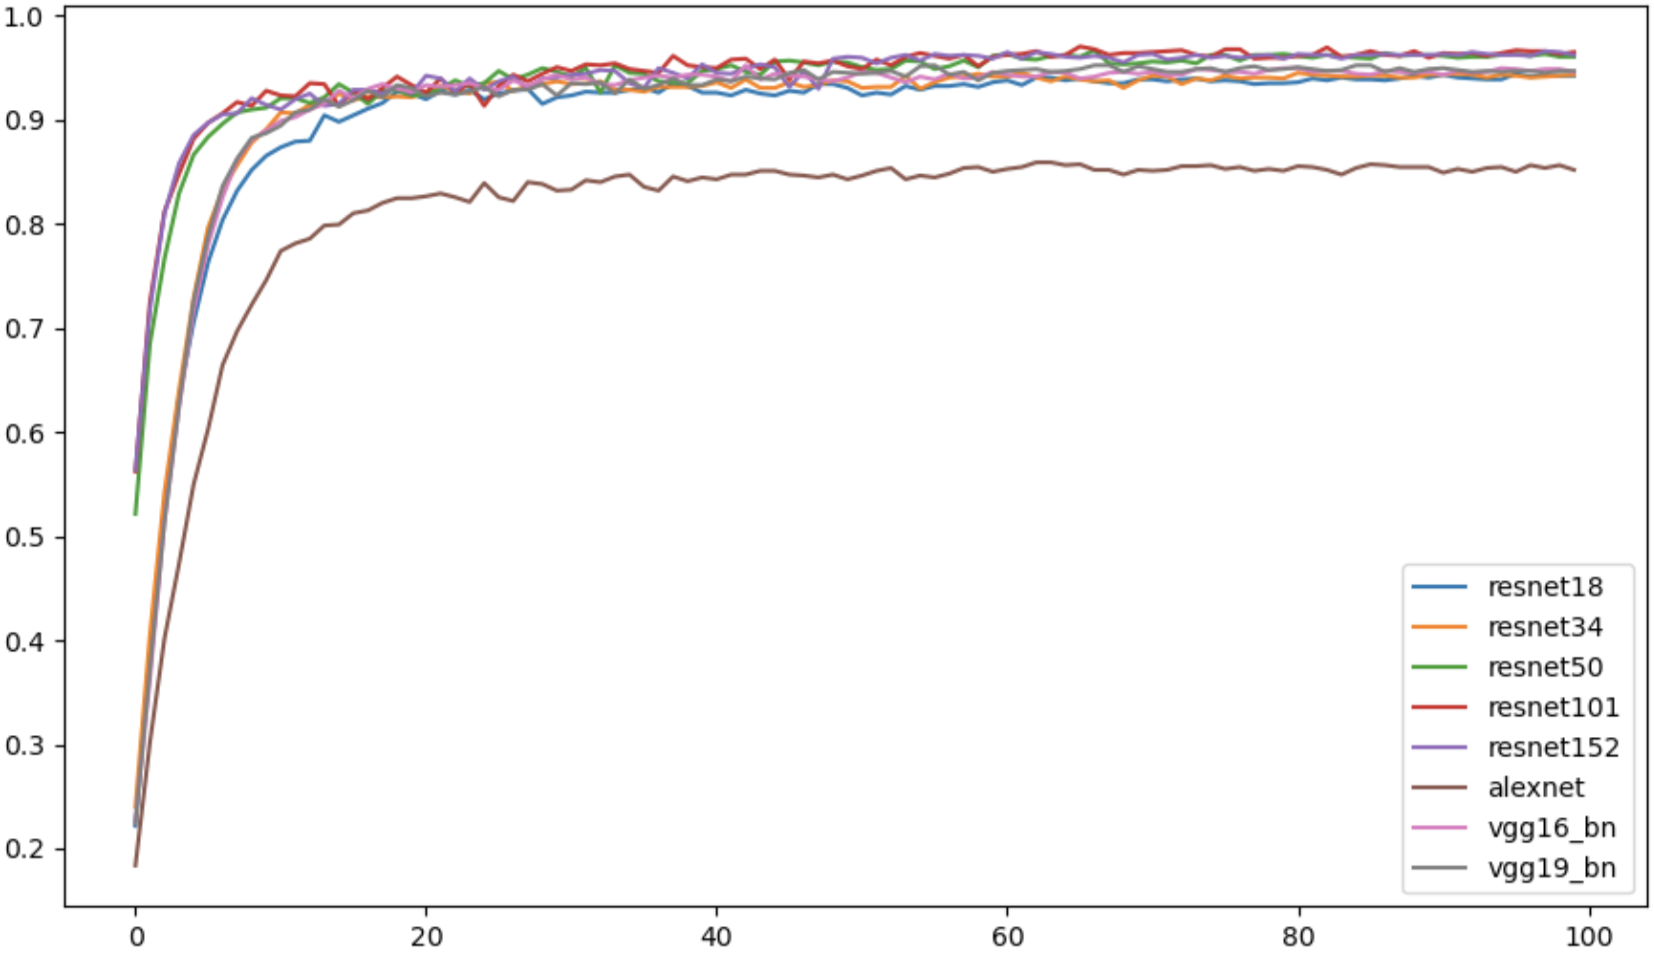
\includegraphics[width = 11 cm]{seedlings_100.png}
        \caption[Accuracy achieved by the models after being trained for 100 epochs]{Accuracy achieved by the models after being trained for 100 epochs. The x axis is the number of epochs, while the y axis is the accuracy achieved}
         \label{fig:seedlings_100_epoch_accuracy}
\end{figure}


\begin{table}[htbp]
\centering
\begin{tabular}{ p{2cm} p{4cm} p{3cm} p{3cm} p{2cm}  }
 Model& Top Accuracy (\%) & Epochs needed &Average Time (s)&Total Time (s)\\
 \hline
Resnet18&94.39&96&7&747\\
Resnet34&94.48&62&9&876\\
Resnet50&96.65&67&14&1439\\
Resnet101&97.01&66&21&2101\\
Resnet152&96.56&98&29&2851\\
Alexnet&85.88&63&7&705\\
VGG16&95.20&43&17&1743\\
VGG19&95.20&56&20&1952\\
 \hline
\end{tabular}
\caption{Performances of the models trained with the 'plant\_seedlings\_v2' dataset for 100 epochs}
\label{tab:performances_seeds}
\end{table}


Fig. \ref{fig:seedlings_100_epoch_accuracy} shows the response of all models during the training based on the epoch used for training. The response of the model shows that, within the first ten epochs, the accuracy increases quickly and tends to stabilise afterwards, increasing slowly over time. However, we can observe a compact graph, meaning all the models (besides Alexnet) achieved accuracies not too far off from each other.
As a matter of fact, the difference in accuracy between the highest performing model (Resnet101) and the lowest performing model (Resnet18) was only 3\%.  


Fig. \ref{fig:seedlings_100_acc}, on the other hand, depicts the accuracy graphed over training time. Alexnet took the least amount of time to finish the training cycle (747 seconds), however Resnet18 took only \textasciitilde40 seconds more and reached a far better accuracy(94\% compared to 85\%). Resnet152 took 47 Minutes and 30 Seconds (2851 seconds) to complete the test and is the model that required the most time. \\
\begin{figure}[h]
       \centering 
	    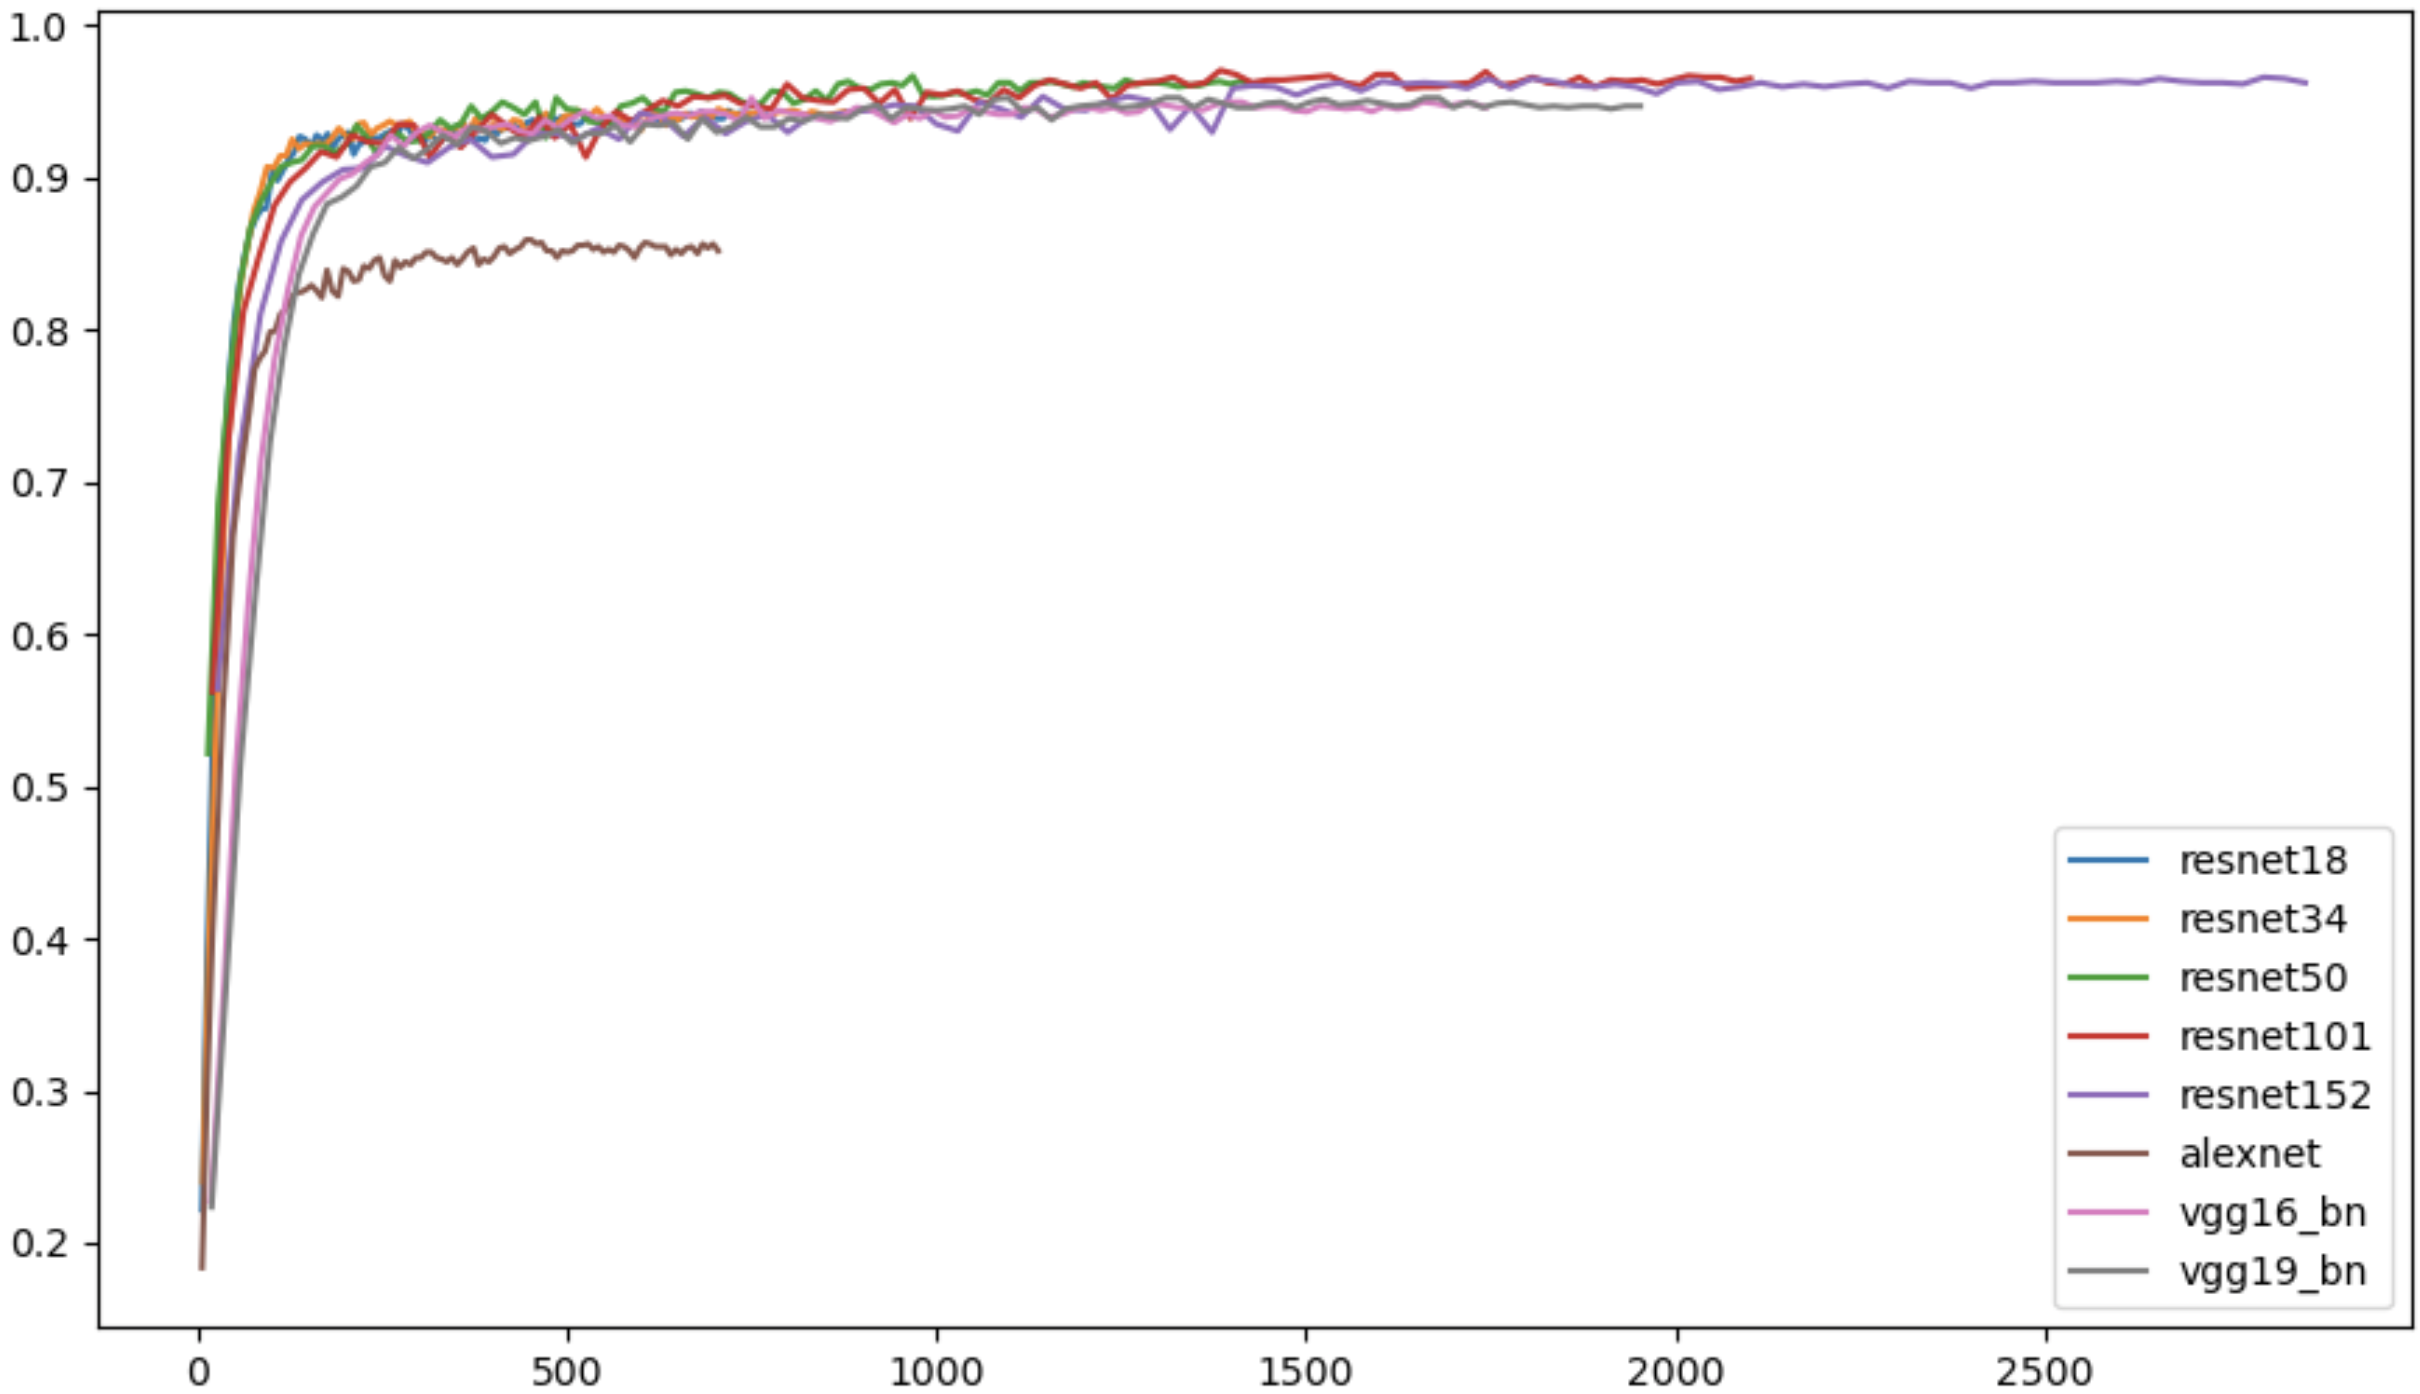
\includegraphics[width = 12 cm]{seedlings_100_acc.png}
        \caption[Accuracy achieved when training for 100 epochs in relation with training time]{Accuracy achieved when training for 100 epochs in relation with training time. The x axis is the training time in seconds, while the y axis is the accuracy achieved}
         \label{fig:seedlings_100_acc}
\end{figure}

\begin{figure}[h]
\begin{subfigure}{0.5\textwidth}
	    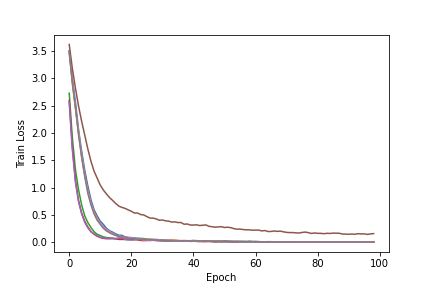
\includegraphics[width = \gws cm]{epoch_train_loss_seeds_100.png}
	    \caption{Training loss calculated over 100 epochs}
        \label{fig:train_loss_seeds_100}
     \end{subfigure} \hfill
     \begin{subfigure}{0.5\textwidth}
	    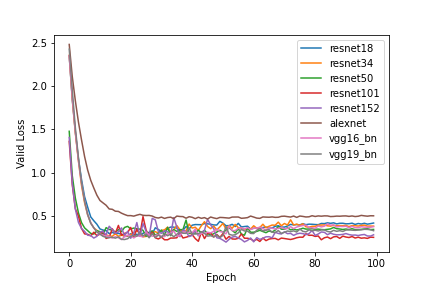
\includegraphics[width = \gws cm]{epoch_valid_loss_seeds_100.png}
	    \caption{Validation loss calculated over 100 epochs}
         \label{fig:valid_loss_seeds_100}
     \end{subfigure}
     
     \caption{Training loss and validation loss of all models calculated over 100 epochs}
        \label{fig:tran_valid_loss_seeds_100}
        
      
\end{figure}


In Fig. \ref{fig:tran_valid_loss_seeds_100}, we can analyse the loss calculated for the models during the training. As shown in Fig. \ref{fig:train_loss_seeds_100}, all the models (besides Alexnet) reached 0 loss within the first 30 epochs. This means that, theoretically, the models learned the dataset perfectly within the first 20 epochs. Usually, when the training loss is 0, we are expecting a case of over-fitting, which would be proven by a high validation loss. We can then study the validation loss of the models in Fig. \ref{fig:valid_loss_seeds_100}. From their response, we can observe that the validation loss does not increase drastically like we saw in the first experiment. On the contrary, we can see in table \ref{tab:difference_val_tra_loss} that the difference between validation loss and training loss is rarely more than 0.4. Furthermore, the curve seems to be quite stable, especially for shallower networks, and the validation loss tends to increase slowly. 
\begin{table}[h]
\centering
        \begin{tabular}{ c c  }
                 Model&Difference\\
                 \hline
                   Resnet18&0.42\\
                    Resnet34&0.38\\
                    Resnet50&0.35\\
                    Resnet101&0.25\\
                    Resnet152&0.28\\
                    Alexnet&0.34\\
                        VGG16&0.38\\
                    VGG19&0.33\\
                    \end{tabular}
                    \caption{Difference between validation loss and train loss after 100 epochs }                   
                     \label{tab:difference_val_tra_loss}
     \end{table} 

For example, we can analyse the trend for the model which reached the highest accuracy overall, namely Resnet101, shown in Fig. \ref{fig:epoch_valid_loss_resnet101}. As shown in table \ref{tab:difference_val_tra_loss}, the difference at the end of the training is 0.25. Moreover - as we suspected before - the training loss approaches zero within the first 30 epochs, while the validation loss remains stable for the entire training process, with some spikes at around the 30 epochs. Furthermore, the validation loss becomes higher than the training loss at around 10 epochs.\\
We can observe a similar behaviour in the response of Resnet152 (Fig. \ref{fig:epoch_valid_loss_resnet152}). The training loss approaches zero once more around the 30 epochs and becomes smaller than the validation loss at around 10. Although the validation loss tends to stabilise for this model, as well, the graph shows a less stable behaviour with more fluctuations between 20 and 50 epochs. \\
\begin{figure}[h]
\begin{subfigure}{0.5\textwidth}
     \centering
	    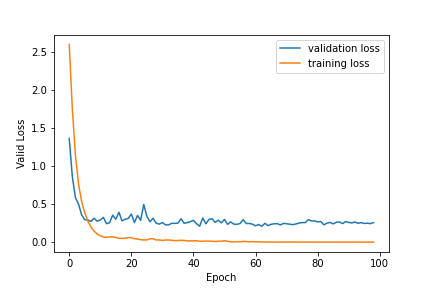
\includegraphics[width = \gws cm]{epoch_valid_loss_resnet101.png}
\caption{Resnet101}\label{fig:epoch_valid_loss_resnet101}
     \end{subfigure}
\begin{subfigure}{0.5\textwidth}
     \centering
	    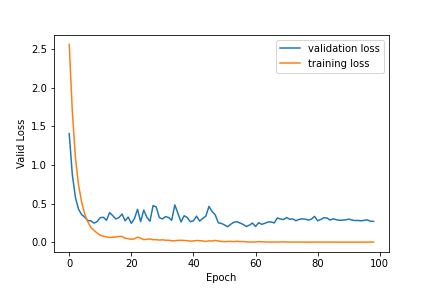
\includegraphics[width = \gws cm]{epoch_valid_loss_resnet152.png}
\caption{Resnet152}\label{fig:epoch_valid_loss_resnet152}
     \end{subfigure}  
     \caption{Training loss and validation loss of Resnet101 and Resnet152 over 100 epochs}
        \label{fig:tran_valid_loss_seeds_res_100}
\end{figure}

In addition to the training time, we can also use the benchmark tool we developed to measure and analyse the inference time of each model.\\
As we are mostly focused on sugar beet recognition, it is safe to assume use cases where field robots would scan the field to recognize the vegetation, similarly to the one proposed by \textit{Lottes et al.} in \cite{7487720}. In such setting, the time taken to classify the image, ultimately, results in a soft deadline, as the time taken to scan the field is greatly influenced by it, therefore being able to estimate the needed inference time could help optimise this part of the application. \\
In order to test for inference time, we are going to use a dataset composed of \textasciitilde120 pictures taken from the original dataset. These pictures were taken before starting the process, therefore they have not been used for training. \\
The results are shown in Fig. \ref{fig:inf_time_epoch_seeds}. Fig. \ref{fig:inf_acc_models_seeds} shows the inference time based on the accuracy, while figure \ref{fig:inf_epoch_models_seeds} shows the inference time based on the epoch used to train. \\
From Fig. \ref{fig:inf_acc_models_seeds} we can start to observe some rather interesting properties. For each model, as they achieve accuracy less than 88\%, the inference time is rarely measured to be more than 60 ms, with only 2 exceptions (\textasciitilde100ms and \textasciitilde390ms). Furthermore, the only model that achieved an accuracy smaller than \textasciitilde82\% is Alexnet\footnote{The whole results can be seen in Fig. \ref{fig:accuracy_inferencetime_seedlings}}.
\begin{figure}[h]
     \begin{subfigure}{0.5\textwidth}
	    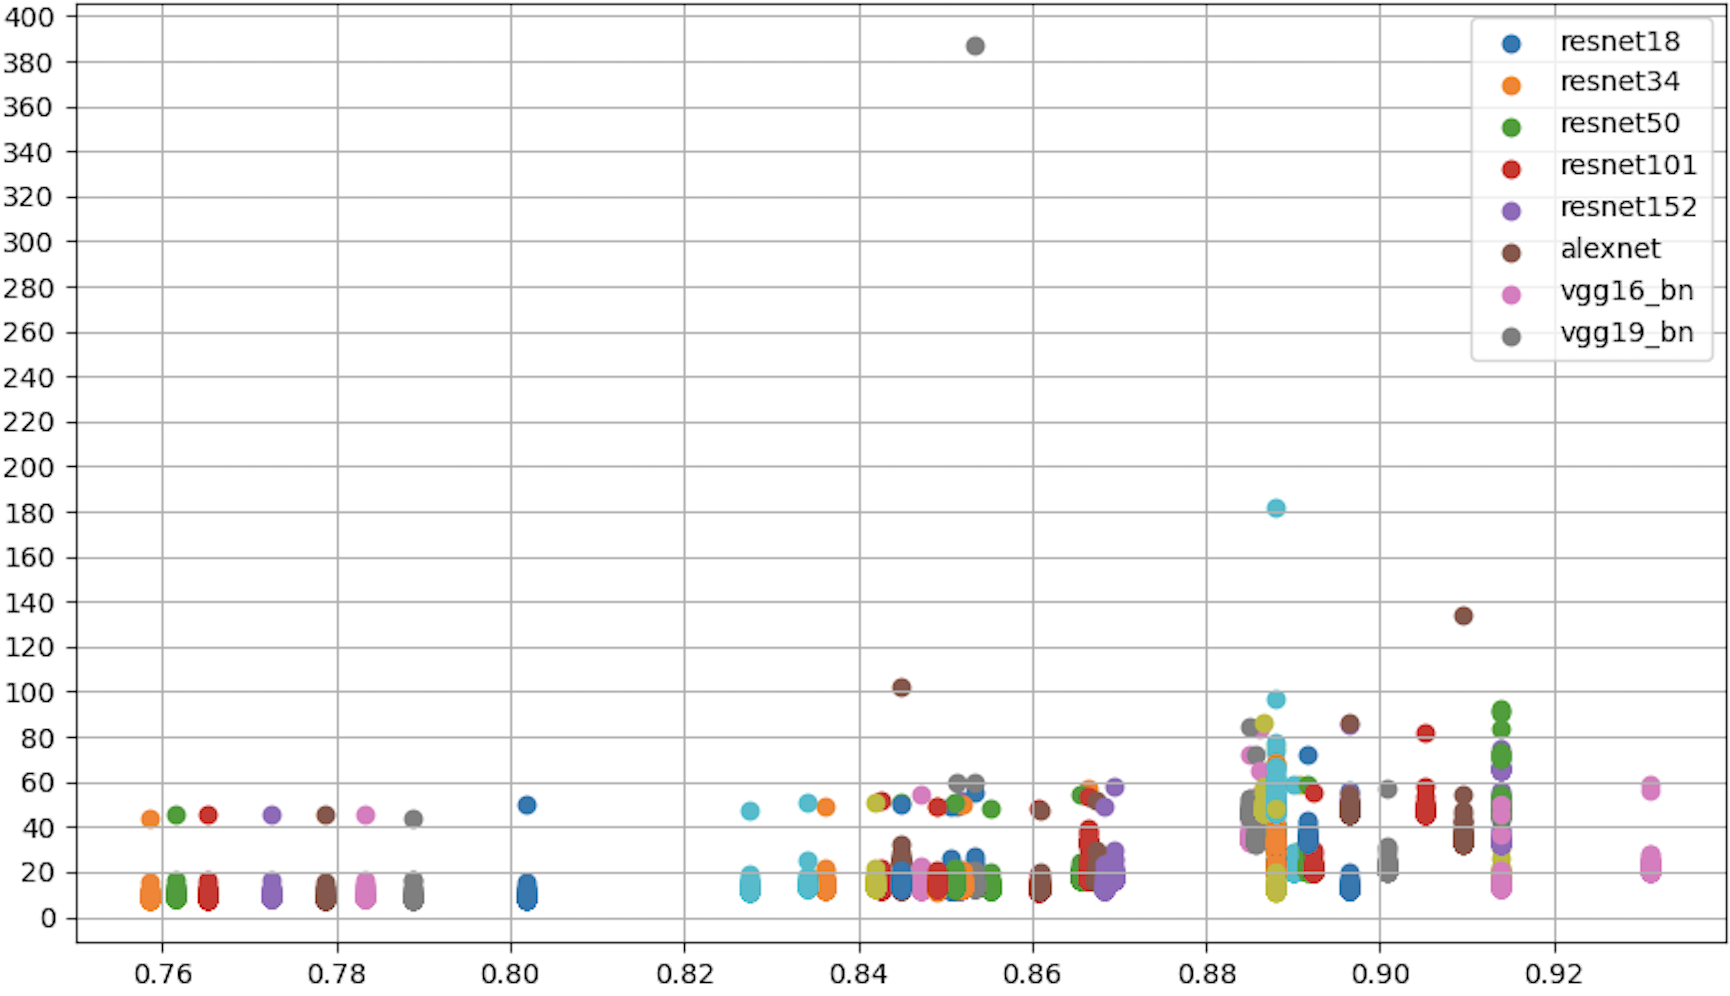
\includegraphics[width = \gws cm]{inf_acc_models_seeds.png}
	    \caption{Based on accuracy}
         \label{fig:inf_acc_models_seeds}
     \end{subfigure}
     \hfill
     \begin{subfigure}{0.5\textwidth}
	    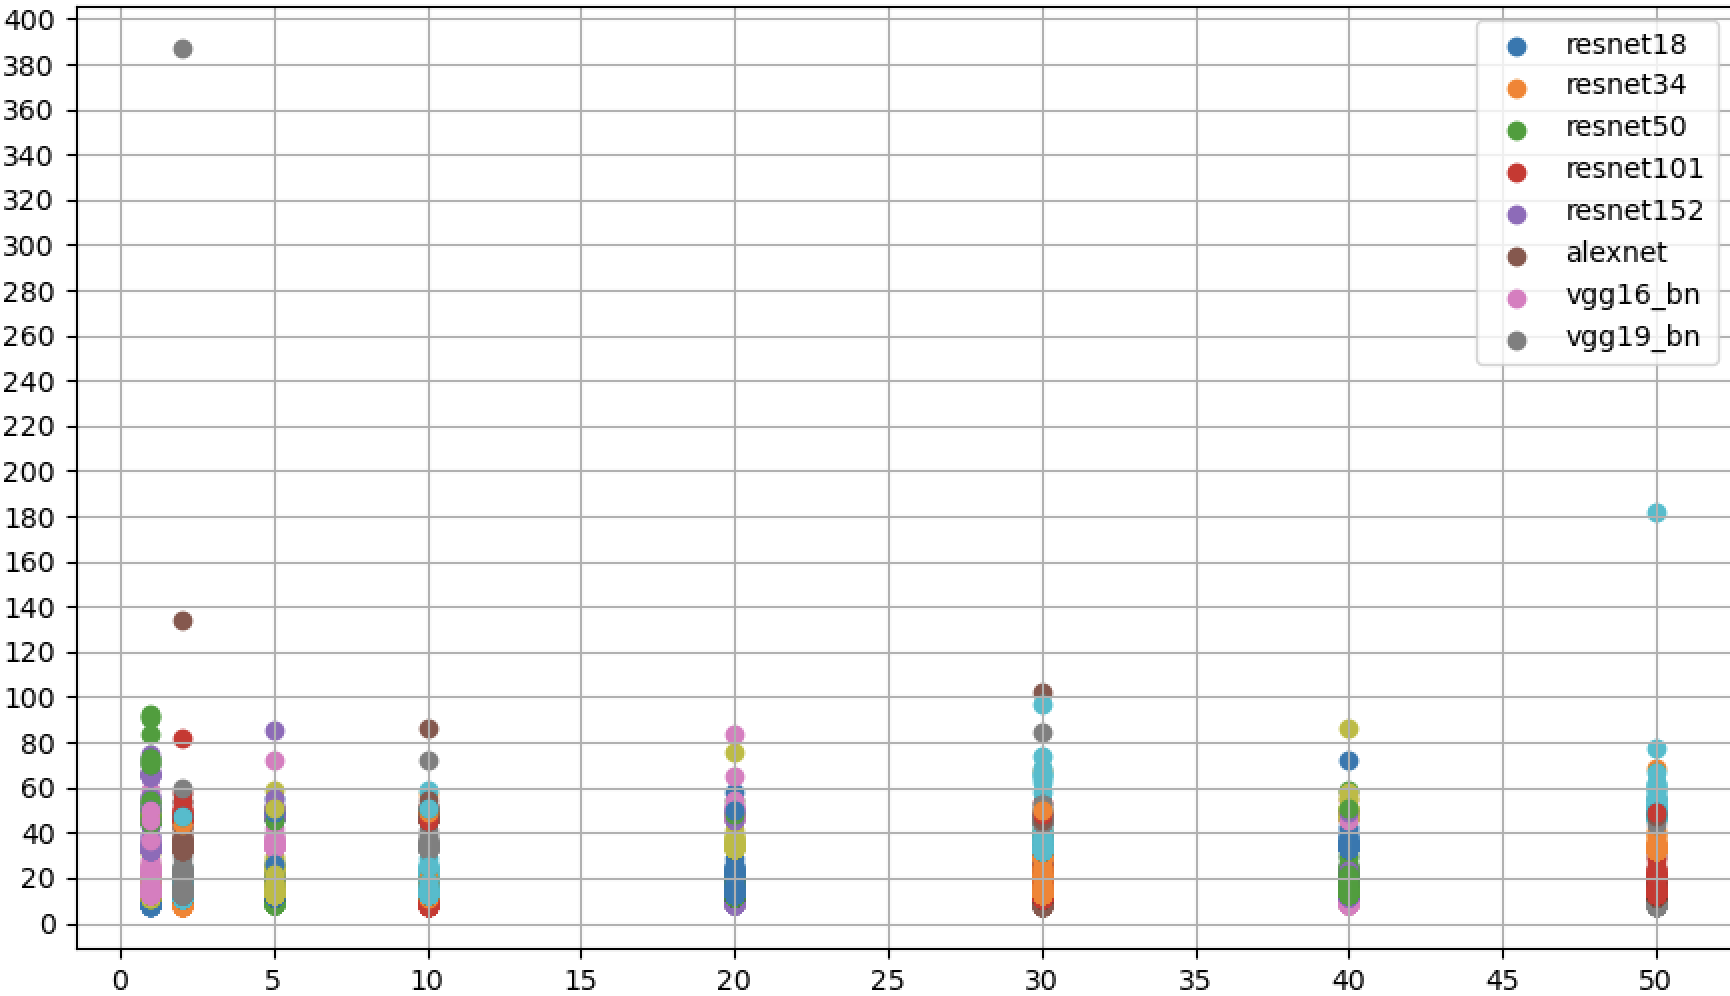
\includegraphics[width = \gws cm]{inf_epoch_models_seeds.png}
	    \caption{Based on the number of epochs}
        \label{fig:inf_epoch_models_seeds}
     \end{subfigure}\\
     \caption[Inference time measured for each model]{Inference time measured for each model using the dataset discussed previously. The inference time is in milliseconds, while the accuracy for Fig. \ref{fig:inf_time_accuracy}is the percentage of correct predictions.}
        \label{fig:inf_time_epoch_seeds}
\end{figure}


For accuracies over 88\%, although the behaviour of the models seems to be less compact, the inference time rarely measures more than 100 milliseconds, with only two outliers(\textasciitilde135ms and \textasciitilde180s).\\
From Fig. \ref{fig:inf_epoch_models_seeds} we can see that, with the exception of the outliers we identified before, the number of epochs that measured the highest value for inference is 30. As a matter of fact, when trained for different numbers of epochs, the models never require more than 100 milliseconds to process the images. 
\begin{figure}[h]
     \begin{subfigure}{0.5\textwidth}
	    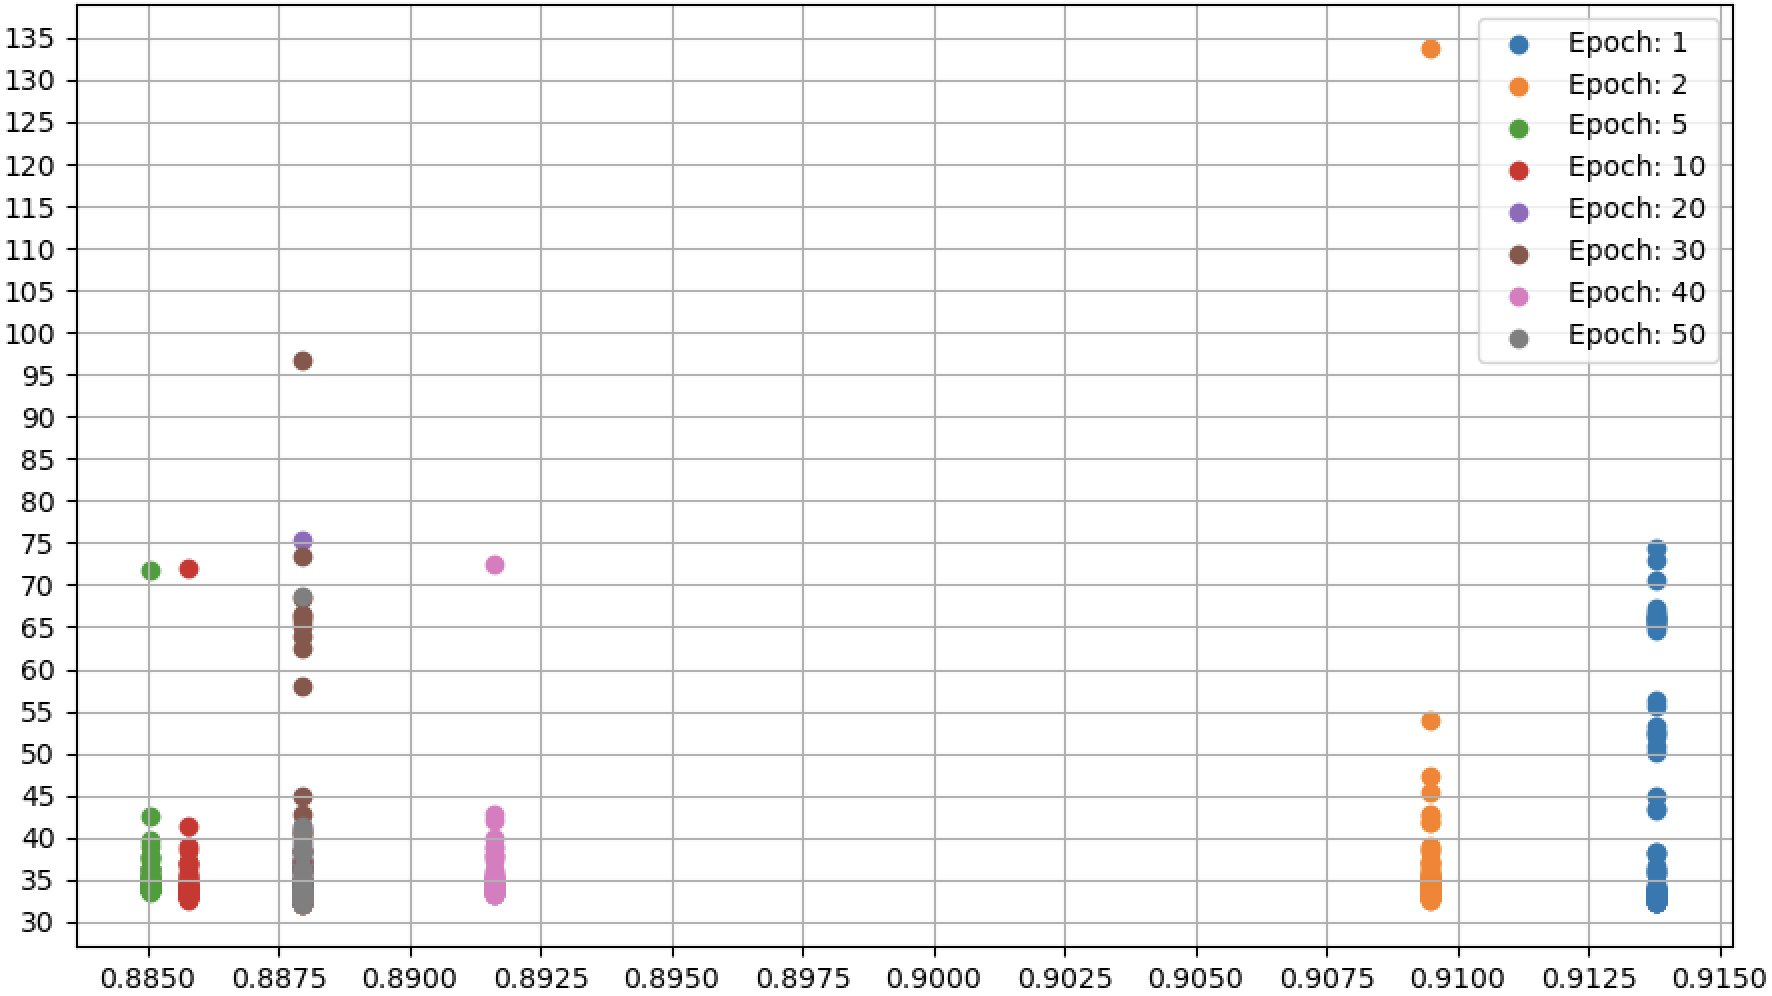
\includegraphics[width = \gws cm]{inf_resnet101_seeds.png}
	    \caption{Resnet101}
         \label{fig:inf_resnet101_seeds}
     \end{subfigure}
     \hfill
     \begin{subfigure}{0.5\textwidth}
	    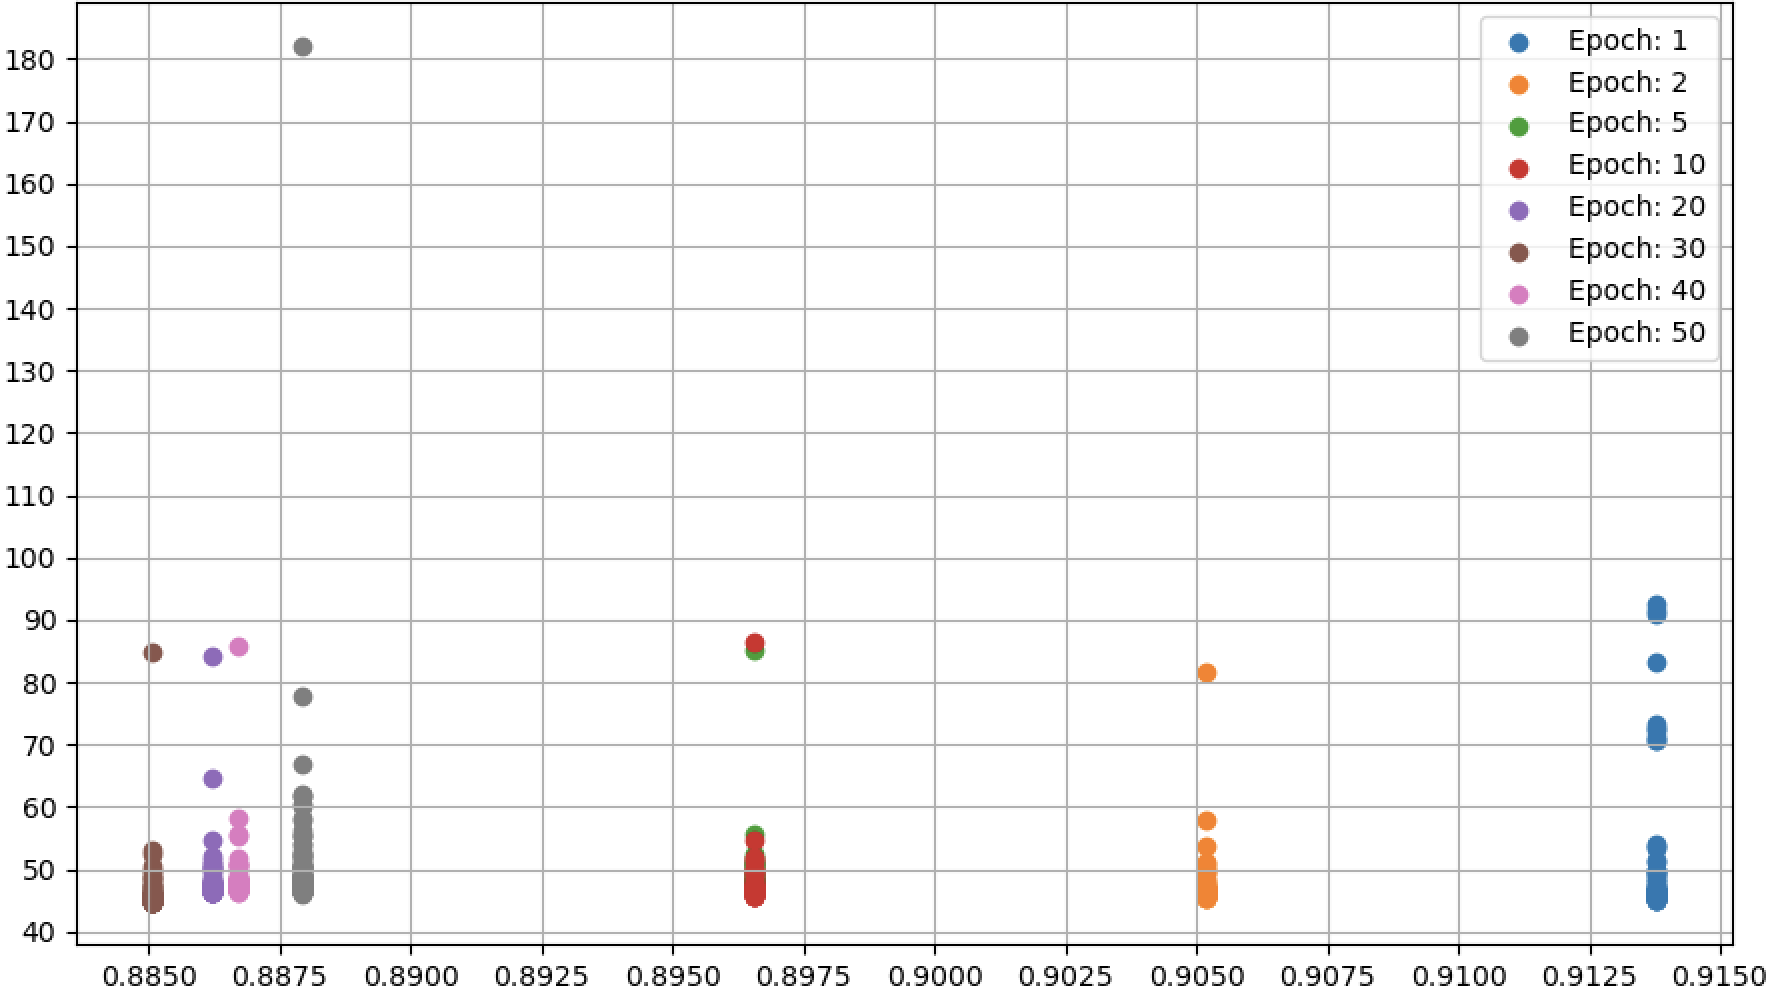
\includegraphics[width = \gws cm]{inf_acc_152_seeds.png}
	    \caption{Resnet152}
        \label{fig:inf_acc_152_seeds}
     \end{subfigure}\\
     \caption[Inference time measured for Resnet101 and Resnet152]{Inference time measured for Resnet101 and Resnet152. The inference time is in milliseconds, while the accuracy is the percentage of correct predictions.}
        \label{fig:inf_time_epoch_seeds2}
\end{figure}



A closer investigation of the individual performance of each model shows further interesting aspects. For the purpose of this experiment, we are going to analyse only Resnet101 and Resnet152, whose behaviour is shown in Fig. \ref{fig:inf_resnet101_seeds} and Fig. \ref{fig:inf_acc_152_seeds} respectively. For both models, we can see that the highest accuracy is achieved when trained for only one (\textasciitilde91\% for both) and two epochs (slightly lower of 91\% for Resnet18 and \textasciitilde90\% for Resnet152). For the other epoch, the accuracy achieved was consistently lower than 90\%. \\
In the case of Resnet101, the fastest training time has been achieved when trained for ten and five epochs, with an inference time of over 45 milliseconds on only two occasions. Although the fastest, the model trained with these epochs also achieved the lowest accuracy. The slowest inference time has been achieved when the model has been trained for two epochs, with an inference as high as 135 milliseconds. However, the model achieved the worst performance when trained for 30 epochs. As a matter of fact, even though it measured the lowest inference time when trained for two epochs, this occurred in only one case, while, when trained for 30 epochs, for a considerable amount of pictures, the inference time was in a range between 57 and 95 milliseconds. \\
Resnet152, on the other hand, showed more consistent results, with an inference time being in the range of 40 to 90 milliseconds for all epochs with the exception of one case where it reached 180 milliseconds. The fastest inference time for this model is measured when the model has been trained for 20 epochs.\\
From this investigation we can conclude that the performances of these two models are quite comparable, when it comes to inference. Both in terms of inference time and accuracy achieved, the two models show similar results, albeit for different levels of training. \\
For example, in the case of Resnet152, with a training time of 580 seconds (20 epochs), we obtain a model that can make predictions in a range between 45 and 85 milliseconds with an accuracy of \textasciitilde89\%. In the case of Resnet101, we can obtain similar results (prediction time between 70 and 30 milliseconds with an accuracy of \textasciitilde89\%) with a training time of 210 seconds (10 epochs). \\

\begin{figure}[h]
       \centering 
	    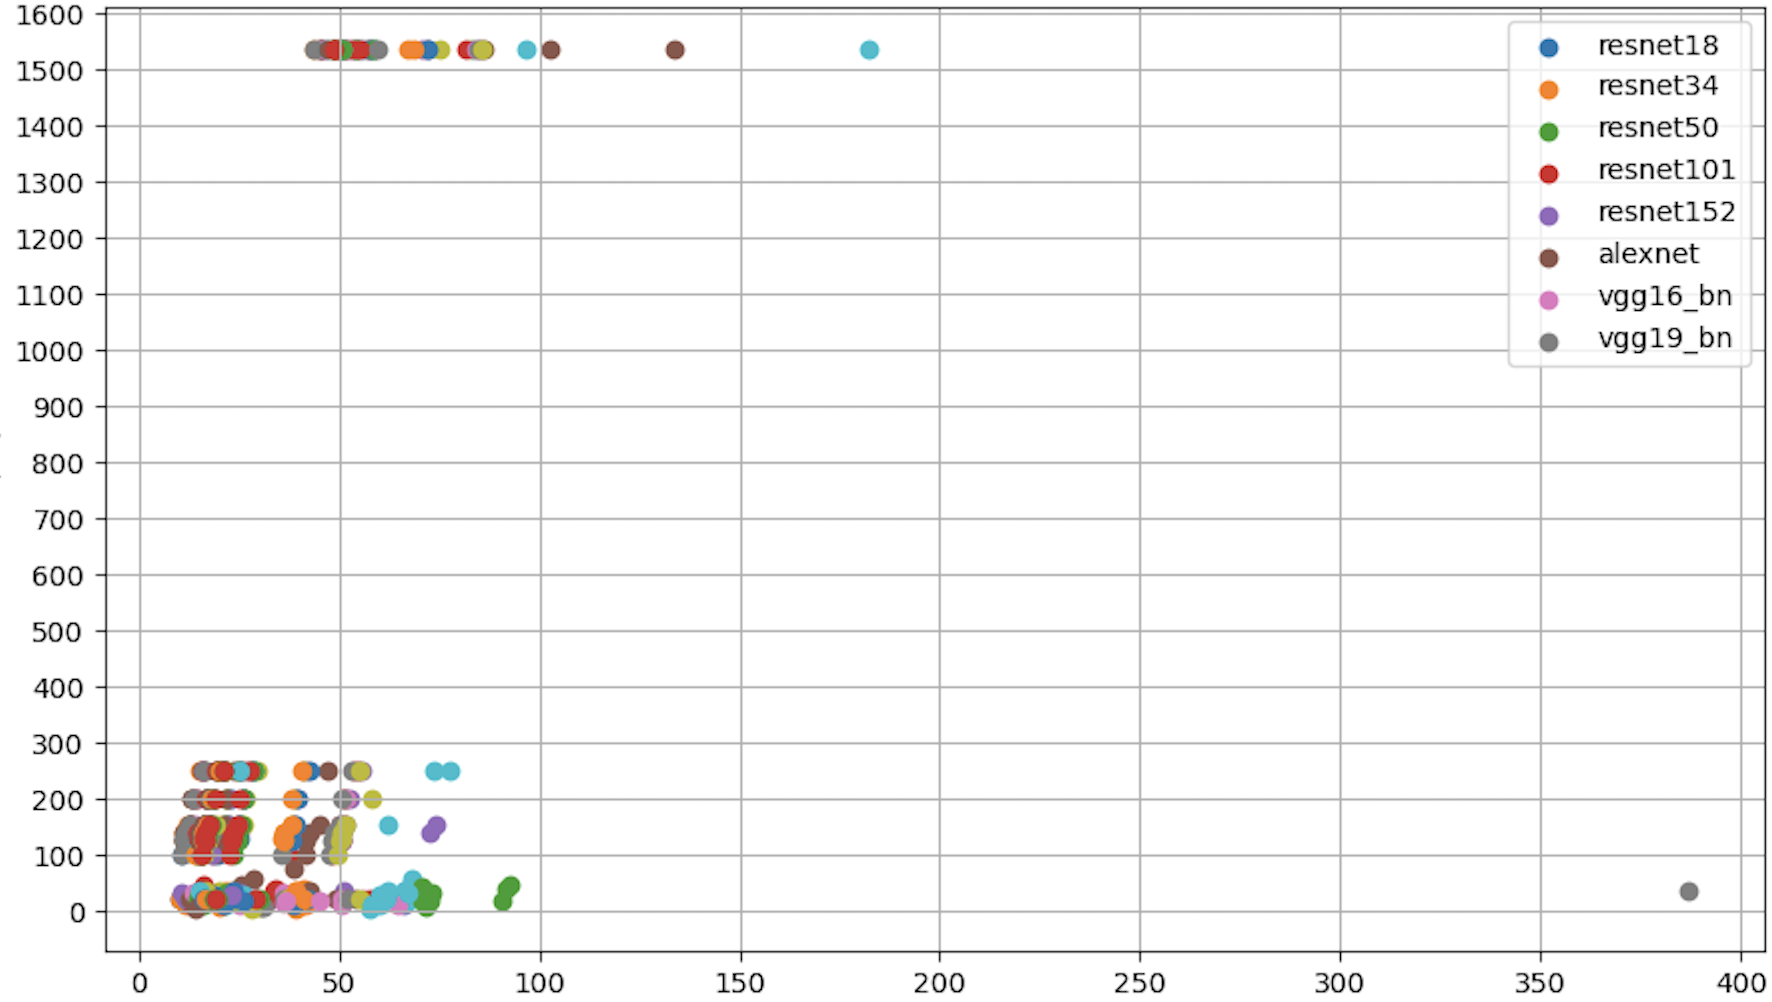
\includegraphics[width = 14 cm]{inf_size_seeds.png}
        \caption[Size of the images over inference time for the seedlings dataset]{This graph shows the size in kb (y axis) of the ten slowest images over the time taken to be processed (x axis)}
         \label{fig:inf_size_seeds}
\end{figure}

We can also run the tool to discover which pictures took the most amount of time to be processed. Fig. \ref{fig:inf_size_seeds} shows the ten slowest images for each model graphed based on their sizes. \\
The graph shows a rather compact and stable behaviour, with the slowest time measured for images having a size bigger than 1500 kb. \\
For pictures of more than 100 kb and less than 300 kb, the inference time is between 0 and 100 ms, with each model performing rather similarly. \\
For this experiment, both for training and for testing inference, we used a dataset with images having rather similar size and resolution, therefore this analysis is not as valuable as expected.\\
However, we can run the tool to make modifications on the images of the dataset. As a matter of fact, the tool also allows one to make a copy of the pictures in the dataset and transform them into grey-scale. Therefore, we can double the amount of pictures in the dataset by including grey-scale copies of those. \\
The results of the first run are shown in table \ref{tab:performances_seeds_gray}. When compared to 
table \ref{tab:performances_seeds}, we can observe that all the models have reached better accuracy besides Alexnet. As a matter of fact, Alexnet peaked at \textasciitilde80\%, while all the other models peaked at accuracies over 95\%. The best accuracy has been achieved by Resnet101 (\textasciitilde99\%) in 80 epochs. Furthermore, this time around, in comparison to the previous run, all the models took more time to train, with a difference in average time for epoch being from one second (Alexnet) to 23 seconds (Resnet152). This is the result of introducing more pictures in the dataset, which makes the training process more time-consuming. \\
\begin{table}[htbp]
\centering
\begin{tabular}{ p{2cm} p{4cm} p{3cm} p{3cm} p{2cm}  }
 Model& Top Accuracy (\%) & Epochs needed &Average Time (s)&Total Time (s)\\
 \hline
Resnet18&95.98&82&9.16&916\\
Resnet34&96.72&90&12.67&1267\\
Resnet50&98.15&82&23.66&2366\\
Resnet101&99.12&80&37.05&3705\\
Resnet152&98.84&85&52.01&5201\\
Alexnet&79.81&89&8.12&812\\
VGG16&97.27&93&29.87&2987\\
VGG19&96.77&64&33.74&3374\\
 \hline
\end{tabular}
\caption{Performance of the models trained for 100 epochs on the 'plant\_seedlings\_v2' dataset including the grey-scale variant of the pictures}
\label{tab:performances_seeds_gray}
\end{table}


The analysis of the training loss and validation loss trends also offers quite different results. An overview can be seen in table \ref{tab:difference_val_tra_loss_2}. The difference in loss between the validation and the training set decreased quite substantially. For example, Resnet101 and Resnet152, which were also the ones with the lowest difference in the previous run (see table \ref{tab:difference_val_tra_loss_2}), measured a difference of only 0.07 and 0.08 respectively. \\
Fig. \ref{fig:tran_valid_loss_seeds_res_100_2} shows the trend for the two models. We can observe that the training loss approaches zero after around 30 epochs, while the validation loss tends to decrease further and stabilises after around 80. It is also worth pointing out that, in the case of Resnet101, the validation loss starts to increase after around 10 epochs and, since the training loss is already approaching zero, it would satisfy the criteria for an early stopping of the training. However, right after the 20 epochs mark, the validation loss decreases once again, up until it becomes only slightly larger than the training and then stabilises afterwards. 

\begin{table}[h]
\centering
        \begin{tabular}{ c c  }
                 Model&Difference\\
                 \hline
                   Resnet18&0.20\\
Resnet34&0.18\\
Resnet50&0.12\\
Resnet101&0.07\\
Resnet152&0.08\\
Alexnet&0.20\\
VGG16&0.12\\
VGG19&0.14\\
                    \end{tabular}
                    \caption{Difference between validation loss and train loss after 100 epochs using the gray-scale variants of the pictures}                   
                     \label{tab:difference_val_tra_loss_2}
     \end{table} 
     
     
\begin{figure}[h]
\begin{subfigure}{0.5\textwidth}
     \centering
	    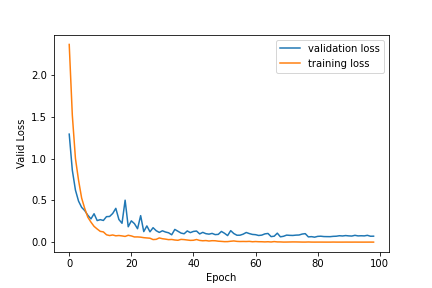
\includegraphics[width = \gws cm]{epoch_valid_loss_resnet101_2.png}
\caption{Resnet101}\label{fig:epoch_valid_loss_resnet101_2}
     \end{subfigure}
\begin{subfigure}{0.5\textwidth}
     \centering
	    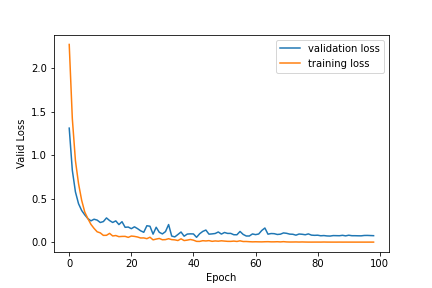
\includegraphics[width = \gws cm]{epoch_valid_loss_resnet152_2.png}
\caption{Resnet152}\label{fig:epoch_valid_loss_resnet152_2}
     \end{subfigure}  
     \caption{Training loss and validation loss of Resnet101 and Resnet152 over 100 epochs on the  'plant\_seedlings\_v2' dataset and the grey-scale variant of the pictures}
        \label{fig:tran_valid_loss_seeds_res_100_2}
\end{figure}
From the information acquired so far, we would expect the models to perform better during the inference time test. Fig. \ref{fig:inf_seeds_with_grey} shows the results of the tests. In Fig. \ref{fig:inf_seeds_grey_no_grey}, the performance of the models has been tested using the same inference dataset we used for the results in Fig. \ref{fig:inf_acc_models_seeds}. Comparing the two graphs, we can observe that the accuracy dropped significantly. As a matter of fact, without the grey images for training, the lowest accuracy achieved was around \textasciitilde75\%, while in this run we calculated accuracies at around \textasciitilde69\%. Furthermore, the highest accuracy calculated in this run is around \textasciitilde88\%,
while in the run before the highest achieved was \textasciitilde92\%. The inference time did not improve as well, as the models showed a comparable or oven worst response time for the images at each epoch. Interestingly, when we observe the overall trend of the models, we can see that as the accuracy increases, it appears that they require more time to process the images and make their predictions.\footnote{The whole results can be seen in Fig. \ref{fig:accuracy_inferencetime_seedlings_grey_train}}\\

\begin{figure}[h]
     \begin{subfigure}{0.5\textwidth}
	    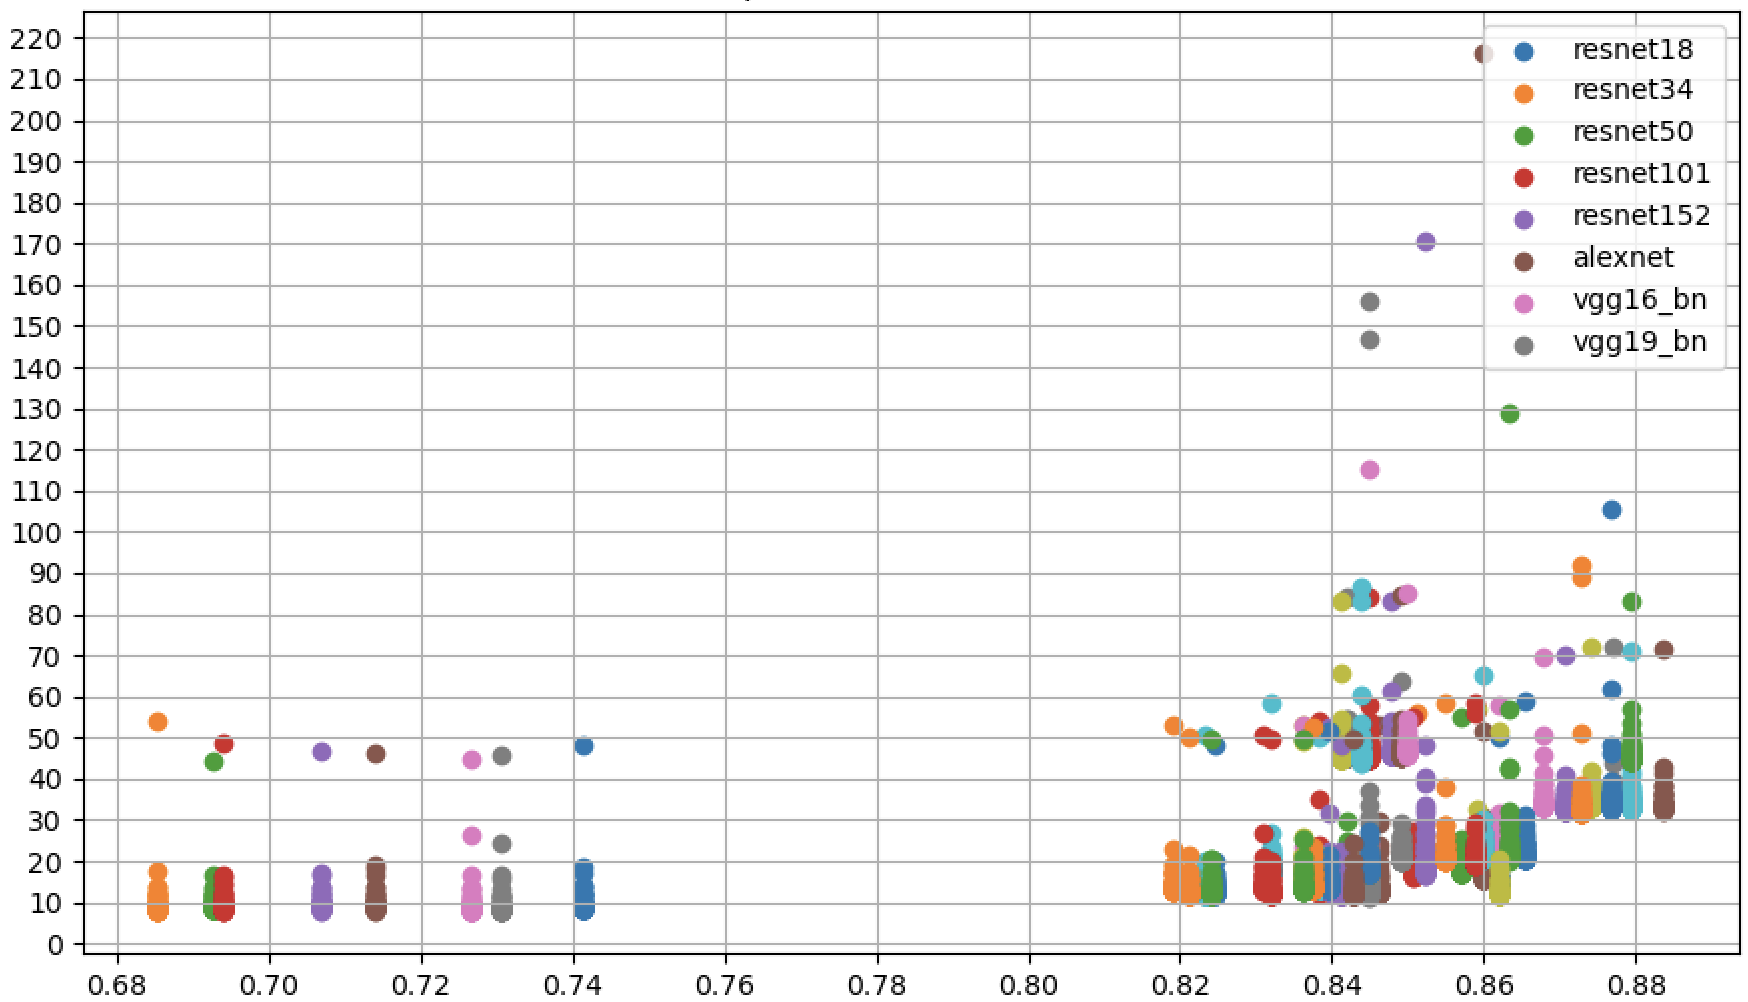
\includegraphics[width = \gws cm]{inf_seeds_grey_no_grey.png}
	    \caption{}
         \label{fig:inf_seeds_grey_no_grey}
     \end{subfigure}
     \hfill
     \begin{subfigure}{0.5\textwidth}
	    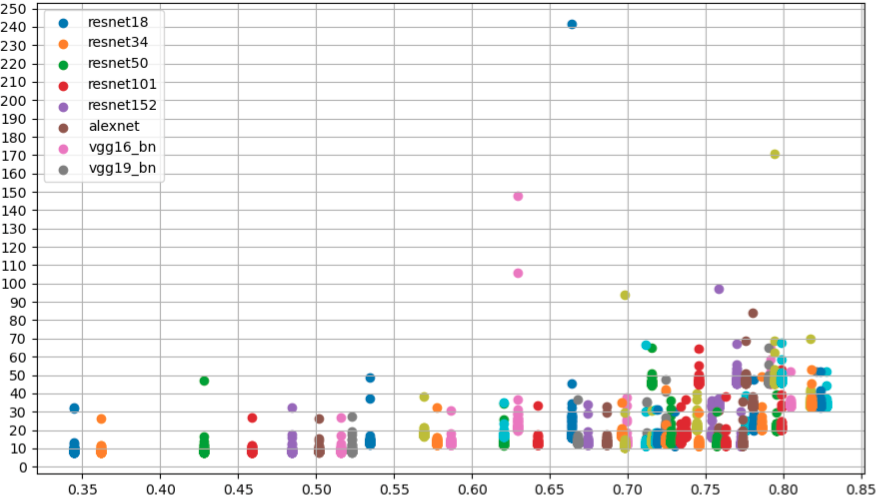
\includegraphics[width = \gws cm]{inf_acc_seeds_grey_img.png}
	    \caption{}
        \label{fig:inf_acc_seeds_grey_img}
     \end{subfigure}\\
     \caption[Inference time of each model trained with grey images as well]{Inference time of each model trained with grey images as well. In Fig. \ref{fig:inf_seeds_grey_no_grey}, the inference is calculated using the same dataset used in Fig. \ref{fig:inf_acc_models_seeds}, while in Fig.  \ref{fig:inf_acc_seeds_grey_img} the dataset is composed with the same pictures, but in grey scale. }
        \label{fig:inf_seeds_with_grey}
\end{figure}


From Fig. \ref{fig:inf_acc_seeds_grey_img},on the other hand, we can see the inference time of the models using the same image we used before, but in grey-scale. In this run, the accuracy dropped to a lowest point of \textasciitilde35\%, a considerable downgrade from the \textasciitilde75\% of the original run. The highest accuracy, on the other hand, dropped to \textasciitilde85\%, i.e. similar to the \textasciitilde88\% of before. In this run, the overall inference time failed to improve, as well, but rather tended to increase as the accuracy increases.\footnote{The whole results can be seen in Fig. \ref{fig:accuracy_inferencetime_seeds_grey}} \\

From these analyses we can conclude that, for this dataset and for these models, including grey-scale versions of the images increases the performances in training, but negatively effects the inference performances of the models. 

\section{Second Experiment}
In this experiment, we are going to use the dataset proposed by \textit{Vevaldi et al.} in \cite{parkhi12a}, which will be referred to as ''the Pets dataset'' for the remainder of this paper. This dataset is directly accessible from the library and contains 37 categories of pets, with roughly 200 pictures each. \\
Even though this dataset contains pictures that are not necessarily related to agriculture, we can use it to obtain information about the behaviour of the models when confronted with images that have different characteristics than the ones we expect. For example, in a farming environment, it is safe to assume that each picture will have similar backgrounds, while this dataset has images with backgrounds that differentiate quite heavily with one another. We can use this dataset, therefore, to compare the results with our first use case, hoping to obtain more useful information.\\
The first metrics we are going to analyse are the number of epochs, training time and accuracy.\\
The benchmarking tool ran the test for each model using three different amounts of epochs, i.e. different training time, in order to simulate three different scenarios: one example with low length of training time, one with a medium length of training time and finally one with a very high length of training time. The tool ran with ten, fifty and a hundred epochs, respectively. \\
The one scenario which yielded more promising results and the one we are going to analyse first is the one with fifty epochs. Fig. \ref{fig:com_ep_ac_models} shows the results of each model's accuracy graphed against the number of epochs used for training, while  Fig. \ref{fig:com_ti_ac_models} shows the results of each model's accuracy graphed against the necessary training time needed to reach that accuracy.\\




\begin{figure}[h]
       \centering 
	    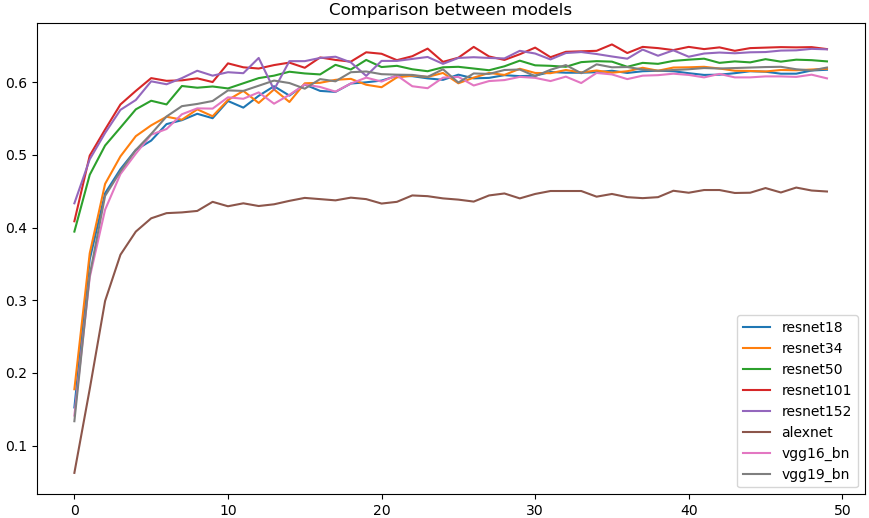
\includegraphics[width = 12 cm]{epoch-accuracy_comparison.png}
        \caption[Comparison between epoch/accuracy for each model]{Comparison between epoch/accuracy for each model. The x axis is the number of epoch, while the y axis is the accuracy achieved}
         \label{fig:com_ep_ac_models}
     \end{figure}
\begin{figure}[h]
\centering 
	    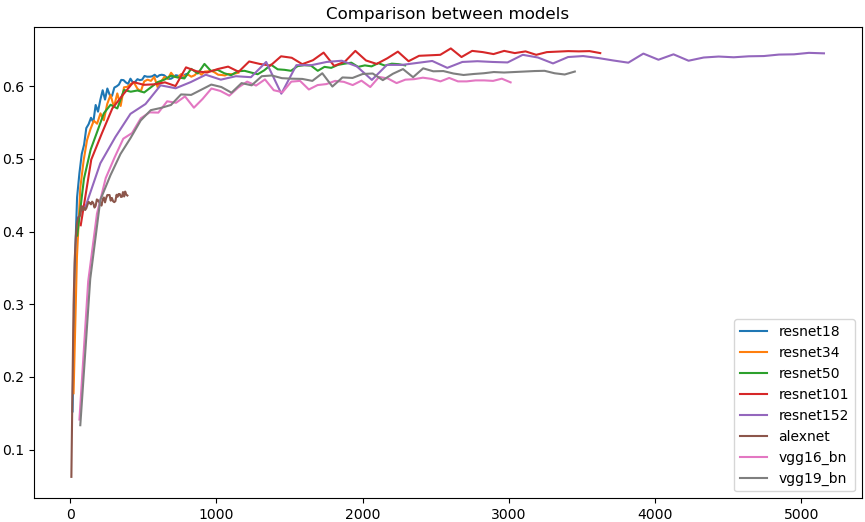
\includegraphics[width = 12 cm]{time-accuracy_comparison.png}
        \caption[Comparison between training time/accuracy for each model]{Comparison between training time/accuracy for each model. The x axis is the training time in seconds, while the y axis is the accuracy achieved}
        \label{fig:com_ti_ac_models}
\end{figure}



As suspected, for each model, the accuracy grows logarithmically higher as the number of  epochs increments, or as the training time increments. A closer inspection of Fig. \ref{fig:com_ti_ac_models} lets us derive other conclusions. Alexnet finishes training in considerably less time compared to the other networks (\textasciitilde 6 minutes), albeit reaching the lowest accuracy overall (45\%). We can observe this difference in time by looking at Fig.\ref{fig:sing_acc_train2} and Fig.\ref{fig:sing_acc_train}, which shows the behaviour of Alexnet, Resnet101, Resnet152 and VGG19 in the same settings. \\
As also shown in the previous graphs, Resnet101 achieved the best overall accuracy at around 65\% with a training time of \textasciitilde 62 minutes, followed by Resnet152, which needed  \textasciitilde 90 minutes to reach an accuracy of \textasciitilde 64\%. Finally, VGG19 took \textasciitilde 60 minutes to reach an accuracy of 61\%. \\
In order to collect more information about the response of the model, we should take a closer look at how they performed individually.\\

\begin{figure}[h]
     \begin{subfigure}{0.5\textwidth}
	    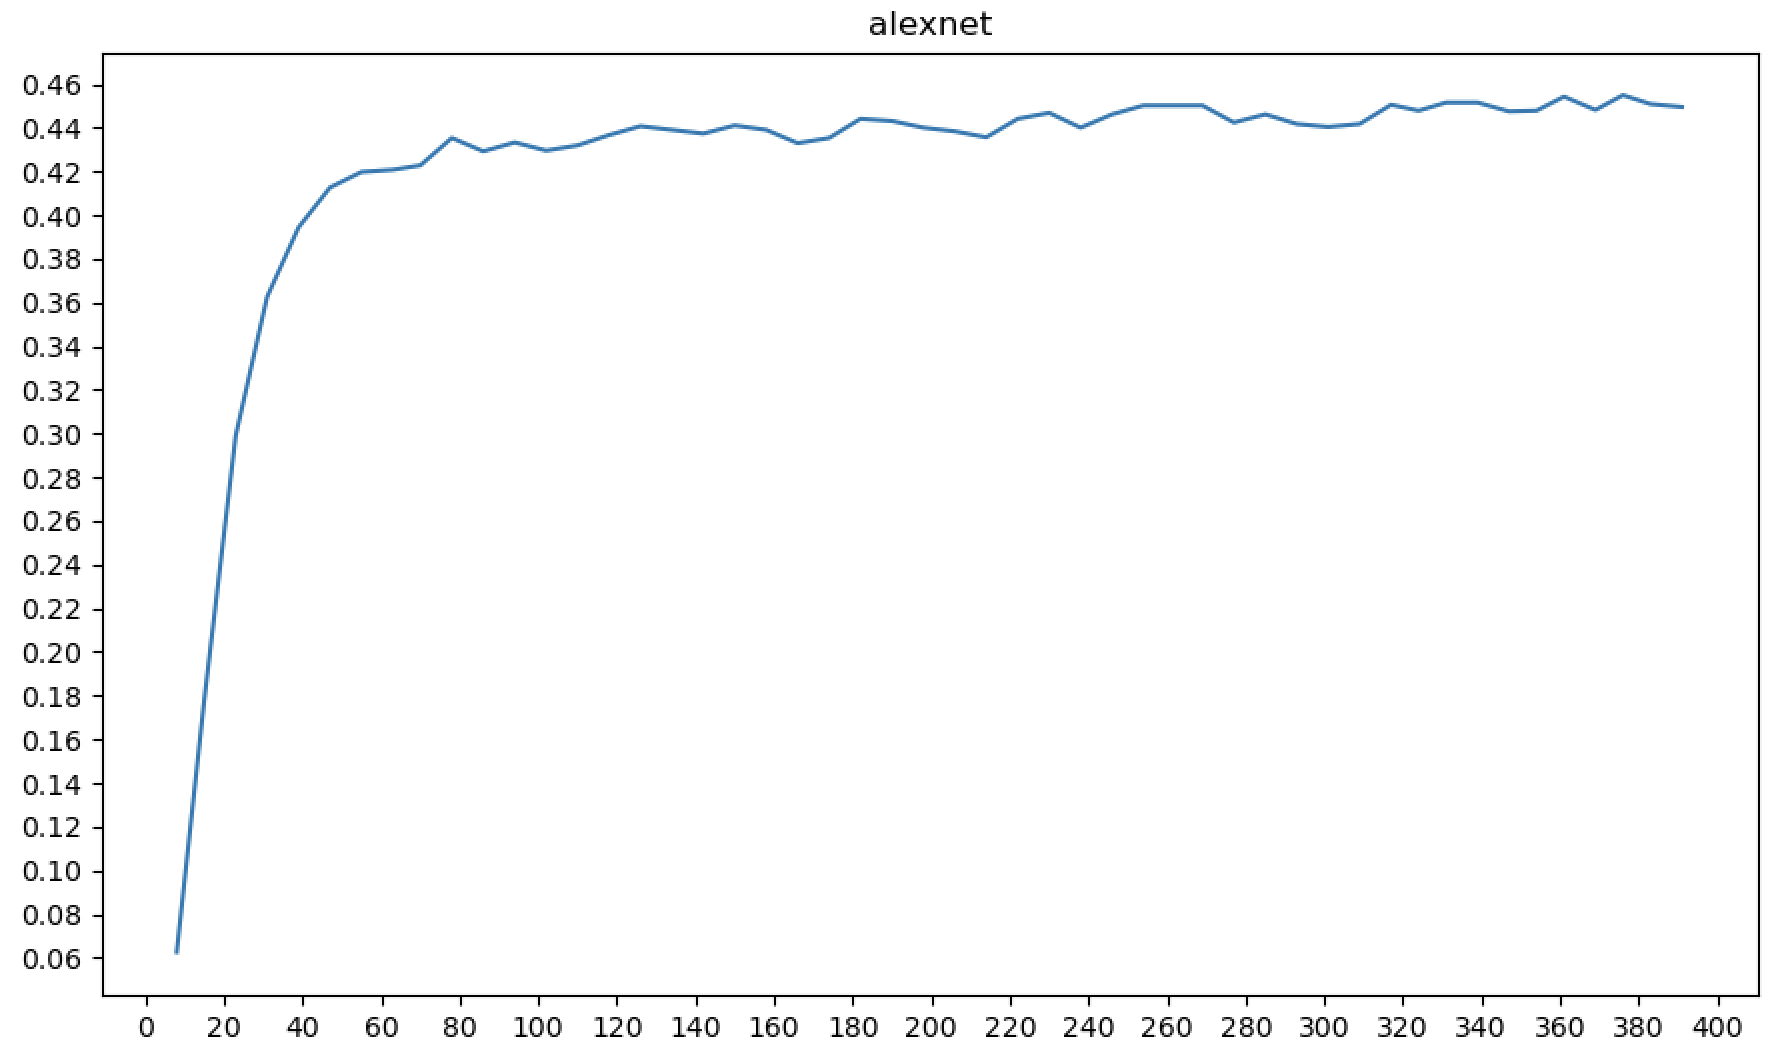
\includegraphics[width = \gws cm]{alexnet_acc_train.png}
         \label{fig:alexnet_acc_train}
     \end{subfigure}
     \hfill
     \begin{subfigure}{0.5\textwidth}
	    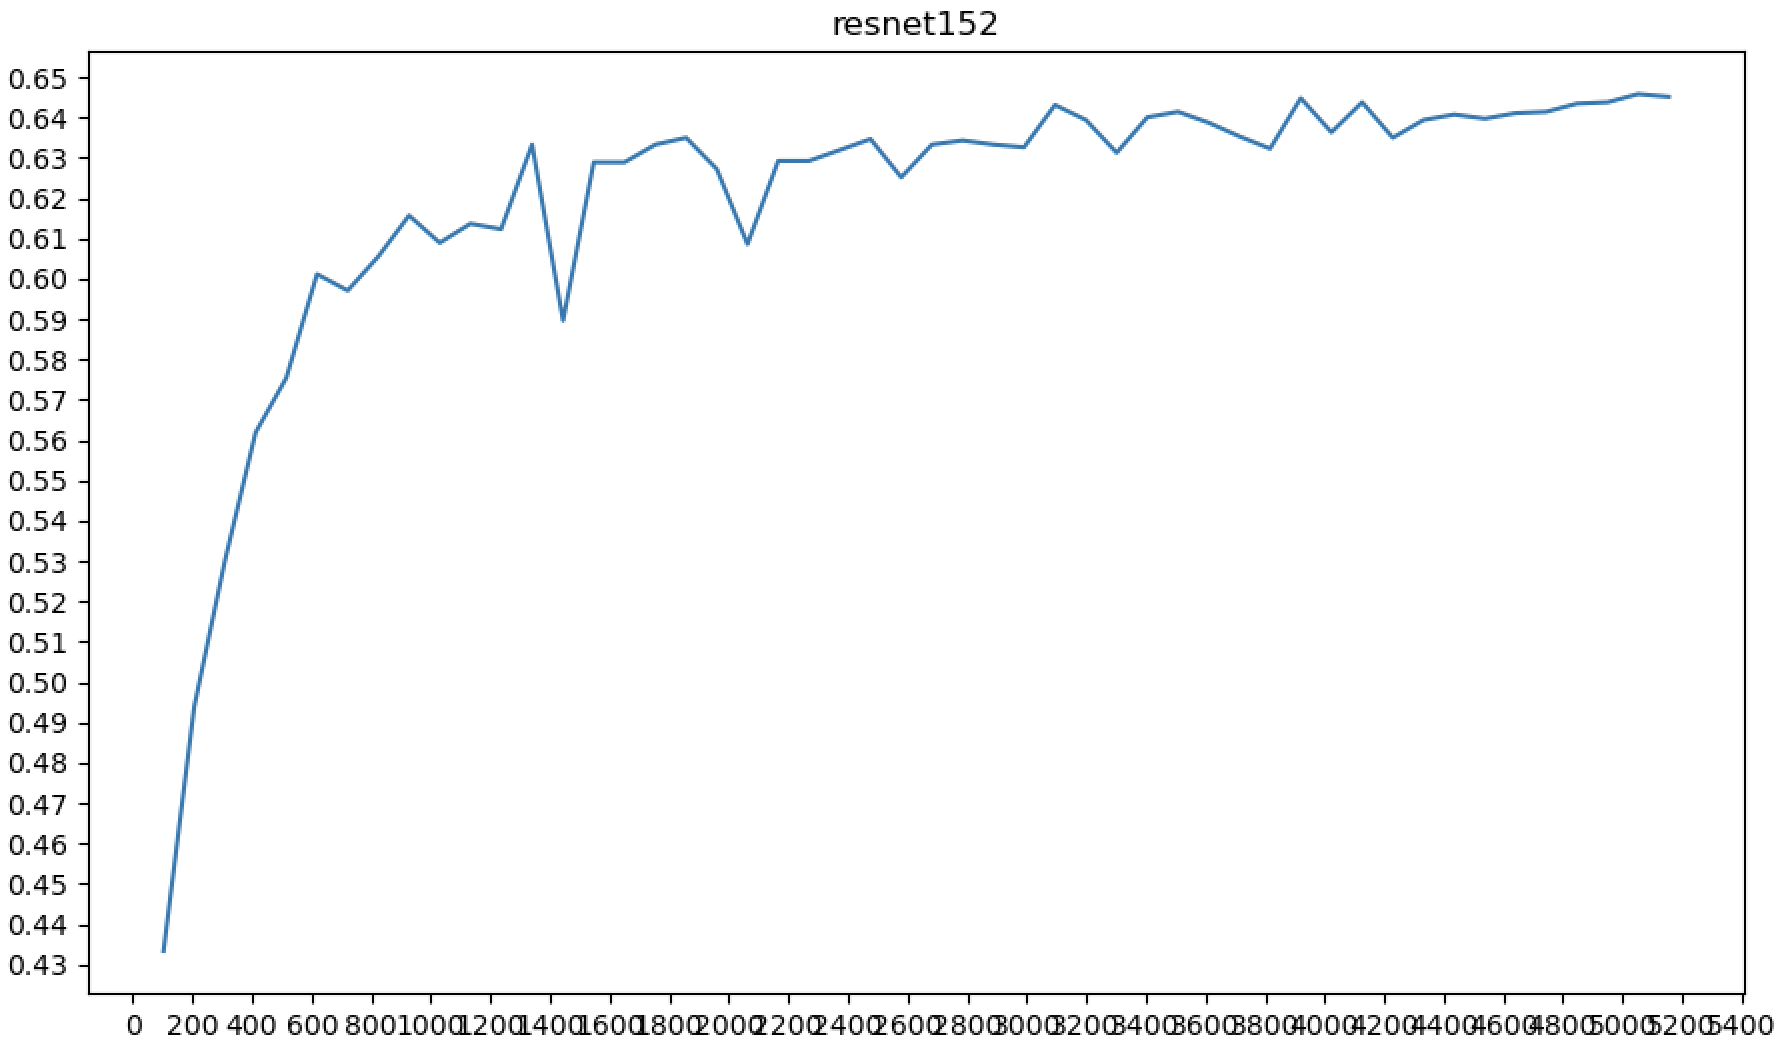
\includegraphics[width = \gws cm]{resnet_152_acc_train.png}
        \label{fig:resnet_152_acc_train}
     \end{subfigure}\\
     \caption{Accuracy of Alexnet and Resnet152 against training time in seconds}
        \label{fig:sing_acc_train2}
\end{figure}
\begin{figure}[h]
     \begin{subfigure}{0.5\textwidth}
	    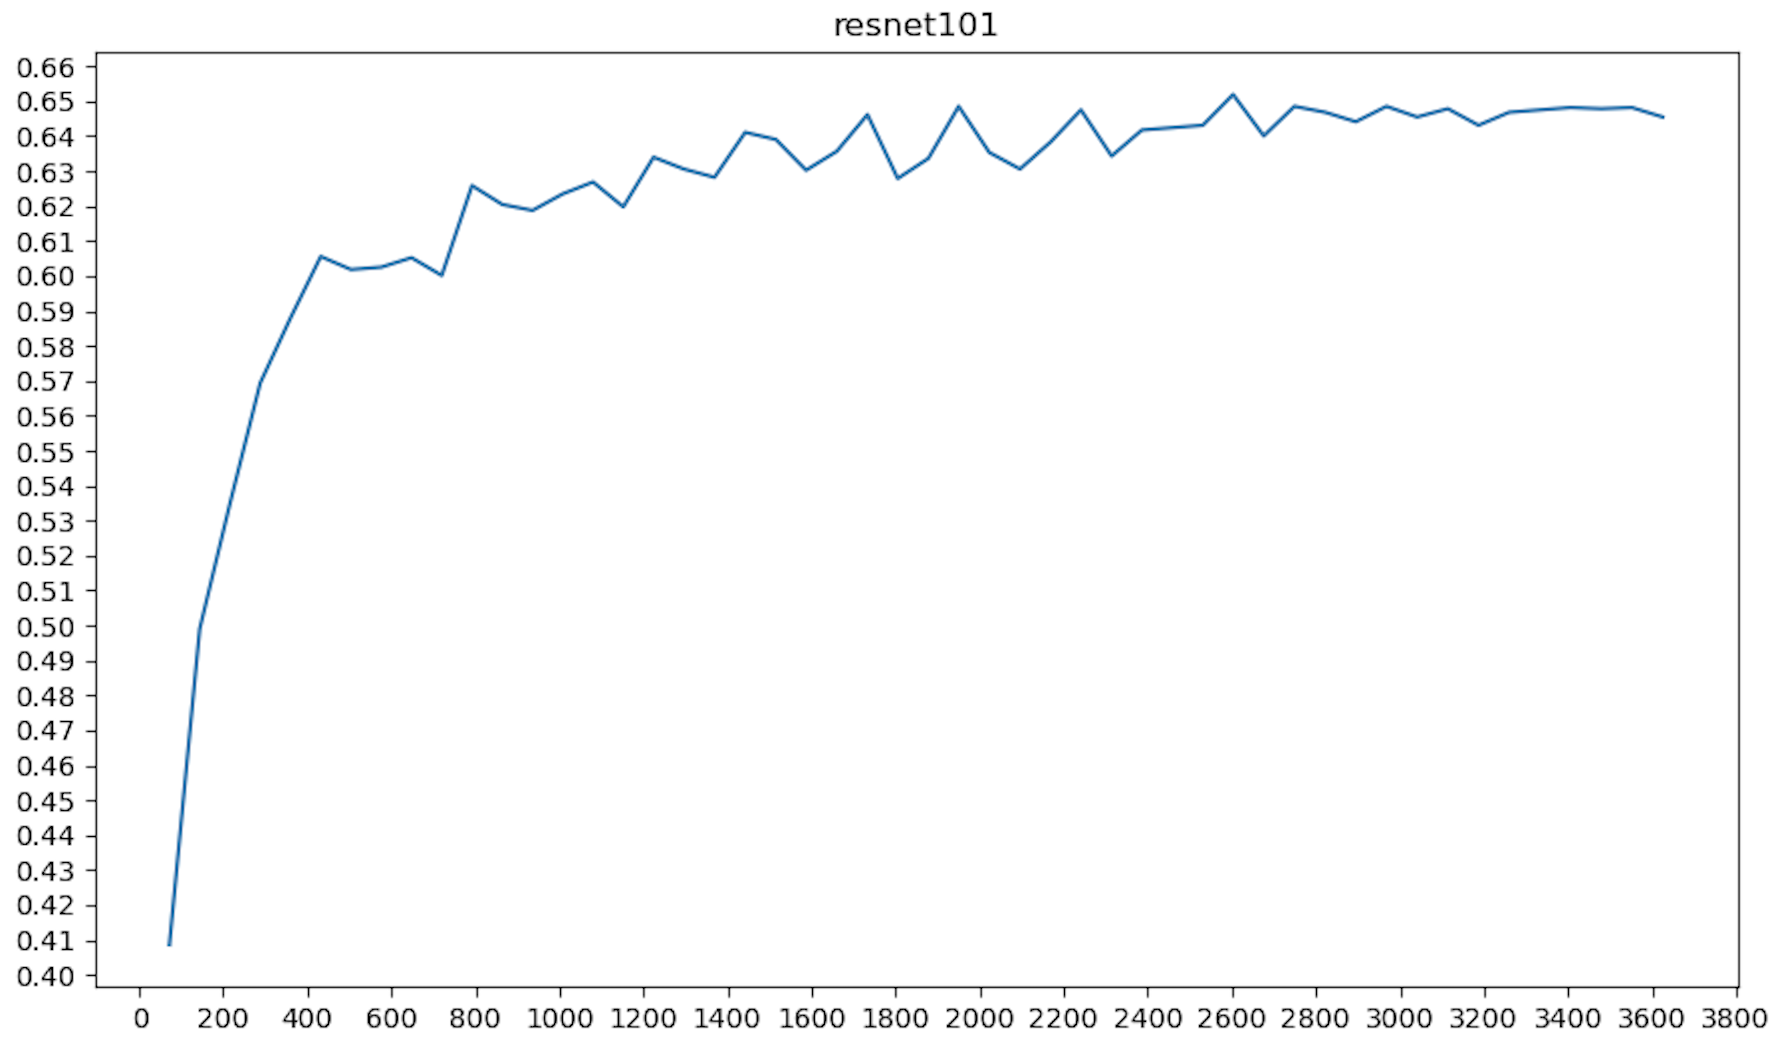
\includegraphics[width = \gws cm]{resnet_101_acc_train.png}
        \label{fig:resnet_1o1_acc_train}
     \end{subfigure}
     \begin{subfigure}{0.5\textwidth}
	    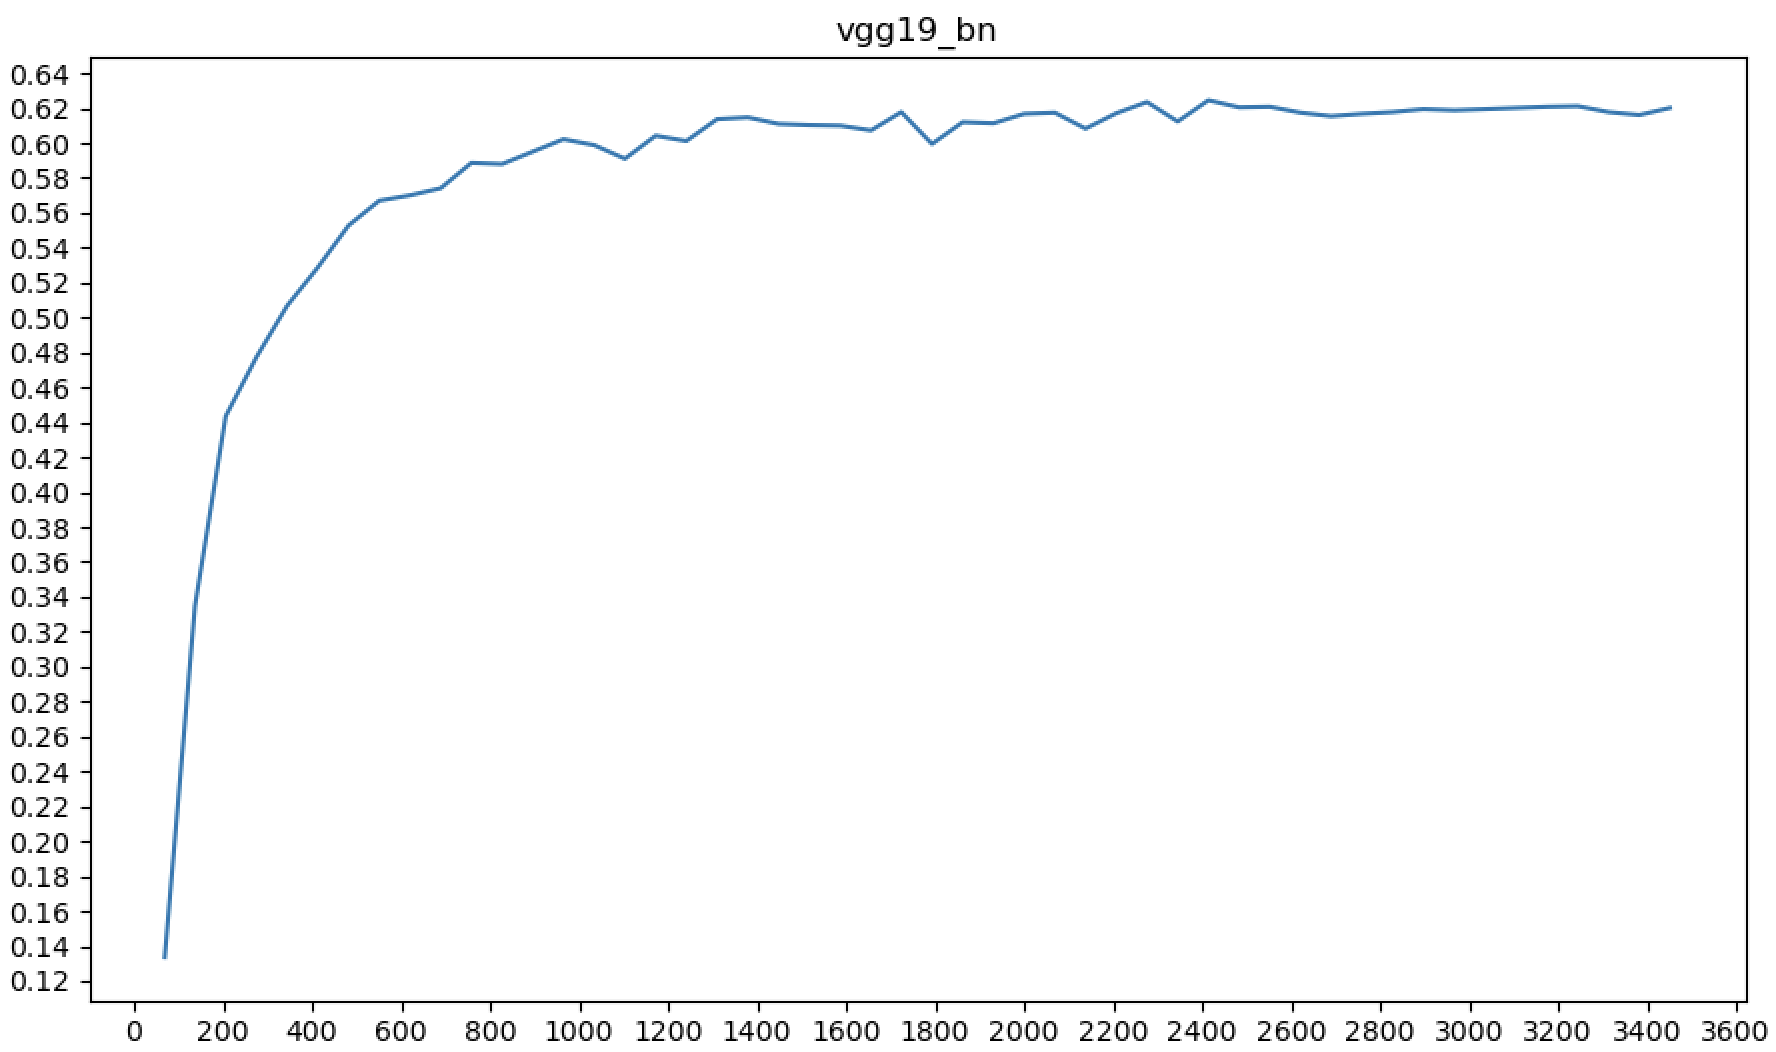
\includegraphics[width = \gws cm]{vgg_19_acc_train.png}
        \label{fig:vgg_19_acc_train}
     \end{subfigure}
        \caption{Accuracy of Resnet101 and VGG9 against training time in seconds}
        \label{fig:sing_acc_train}
\end{figure}
Fig.\ref{fig:sing_acc_train2} and Fig.\ref{fig:sing_acc_train} also show how stable each model was during training. The stability we are observing, in this instance, is how fluctuating each model has been during training, regarding its accuracy. The less fluctuating it is, the better we able to predict the accuracy from the training time, or the number of epochs, and vice-versa. From the results, we can see that Resnet152 and Resnet101 tend to fluctuate more compared to Alexnet or VGG19 (Fig. \ref{fig:sing_acc_train}). \\
Such fluctuation, however, does not hide a trend which is common amongst all models: after a certain number of epochs, the accuracy tends to stabilise and grow significantly slower. Fig. \ref{fig:com_ep_ac_models} can help us locate the point at which the accuracy stops increasing at a high rate at around 10 epochs and this is further proved by Fig. \ref{fig:sing_acc_ep}.\\
\begin{figure}[h]
     \begin{subfigure}{0.5\textwidth}
	    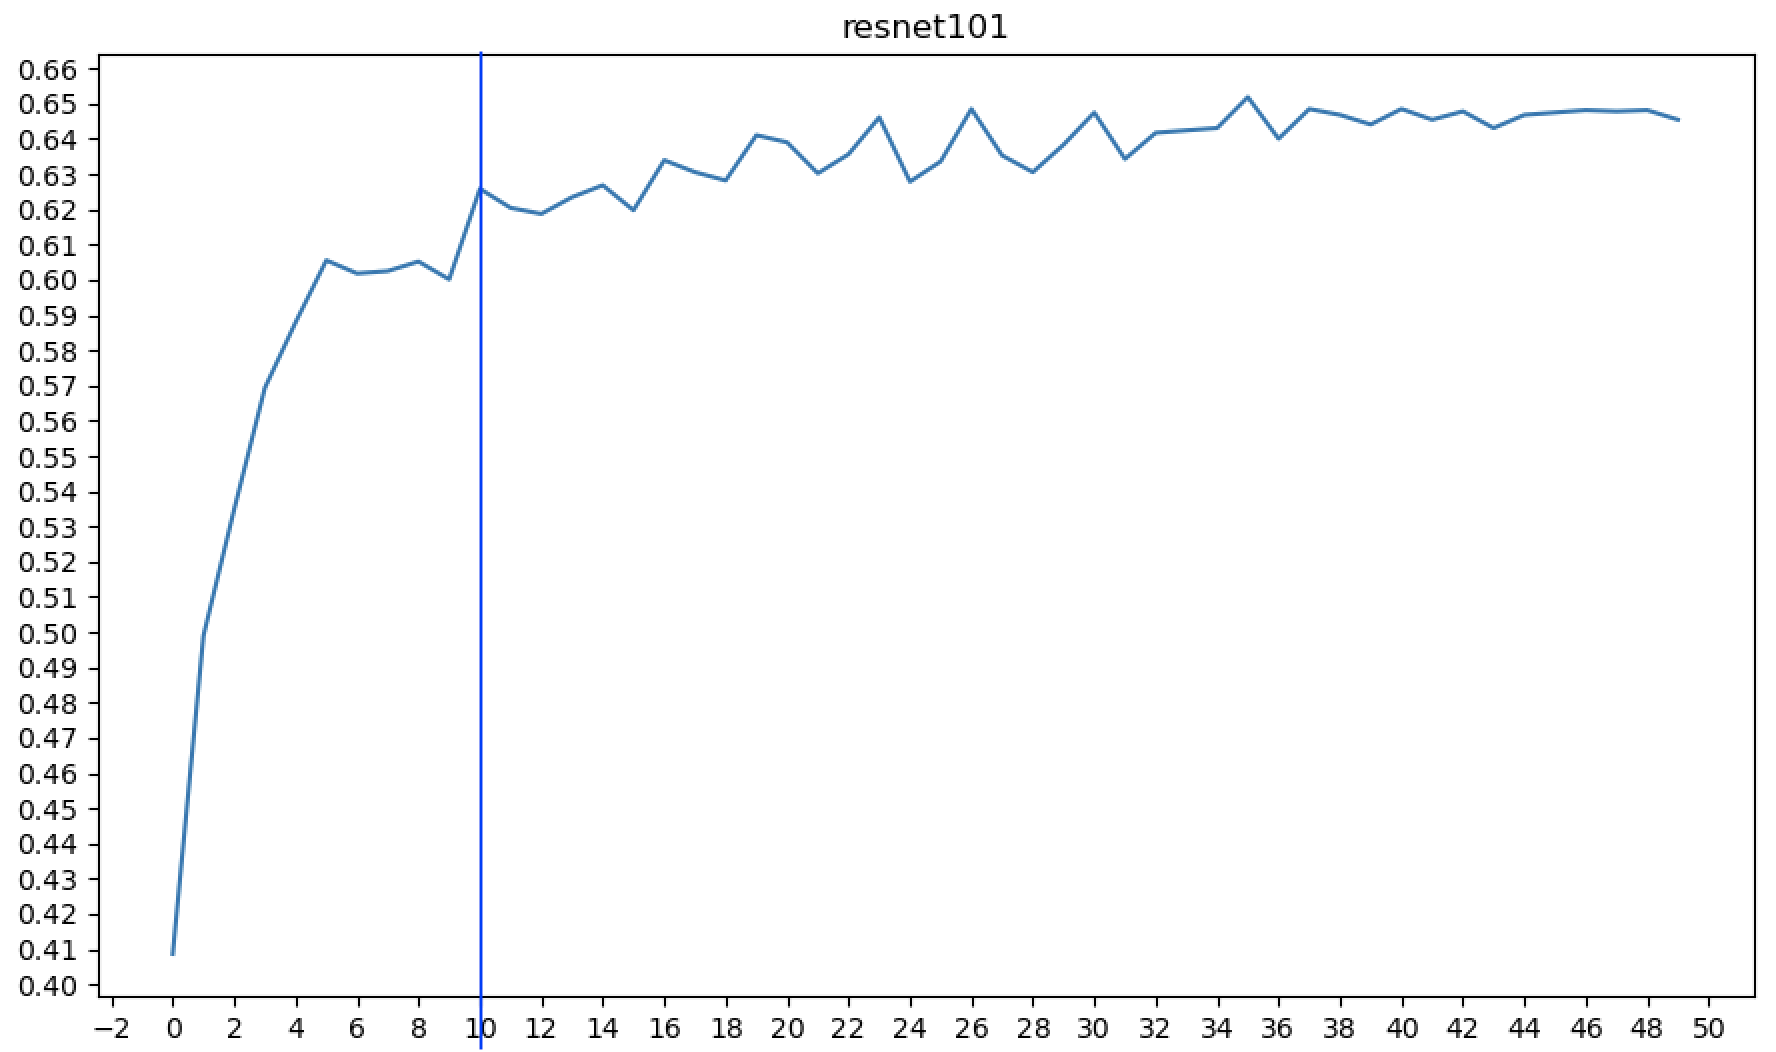
\includegraphics[width = \gws cm]{resnet_101_acc_ep.png}
        \label{fig:resnet_101_acc_ep}
     \end{subfigure}
     \begin{subfigure}{0.5\textwidth}
	    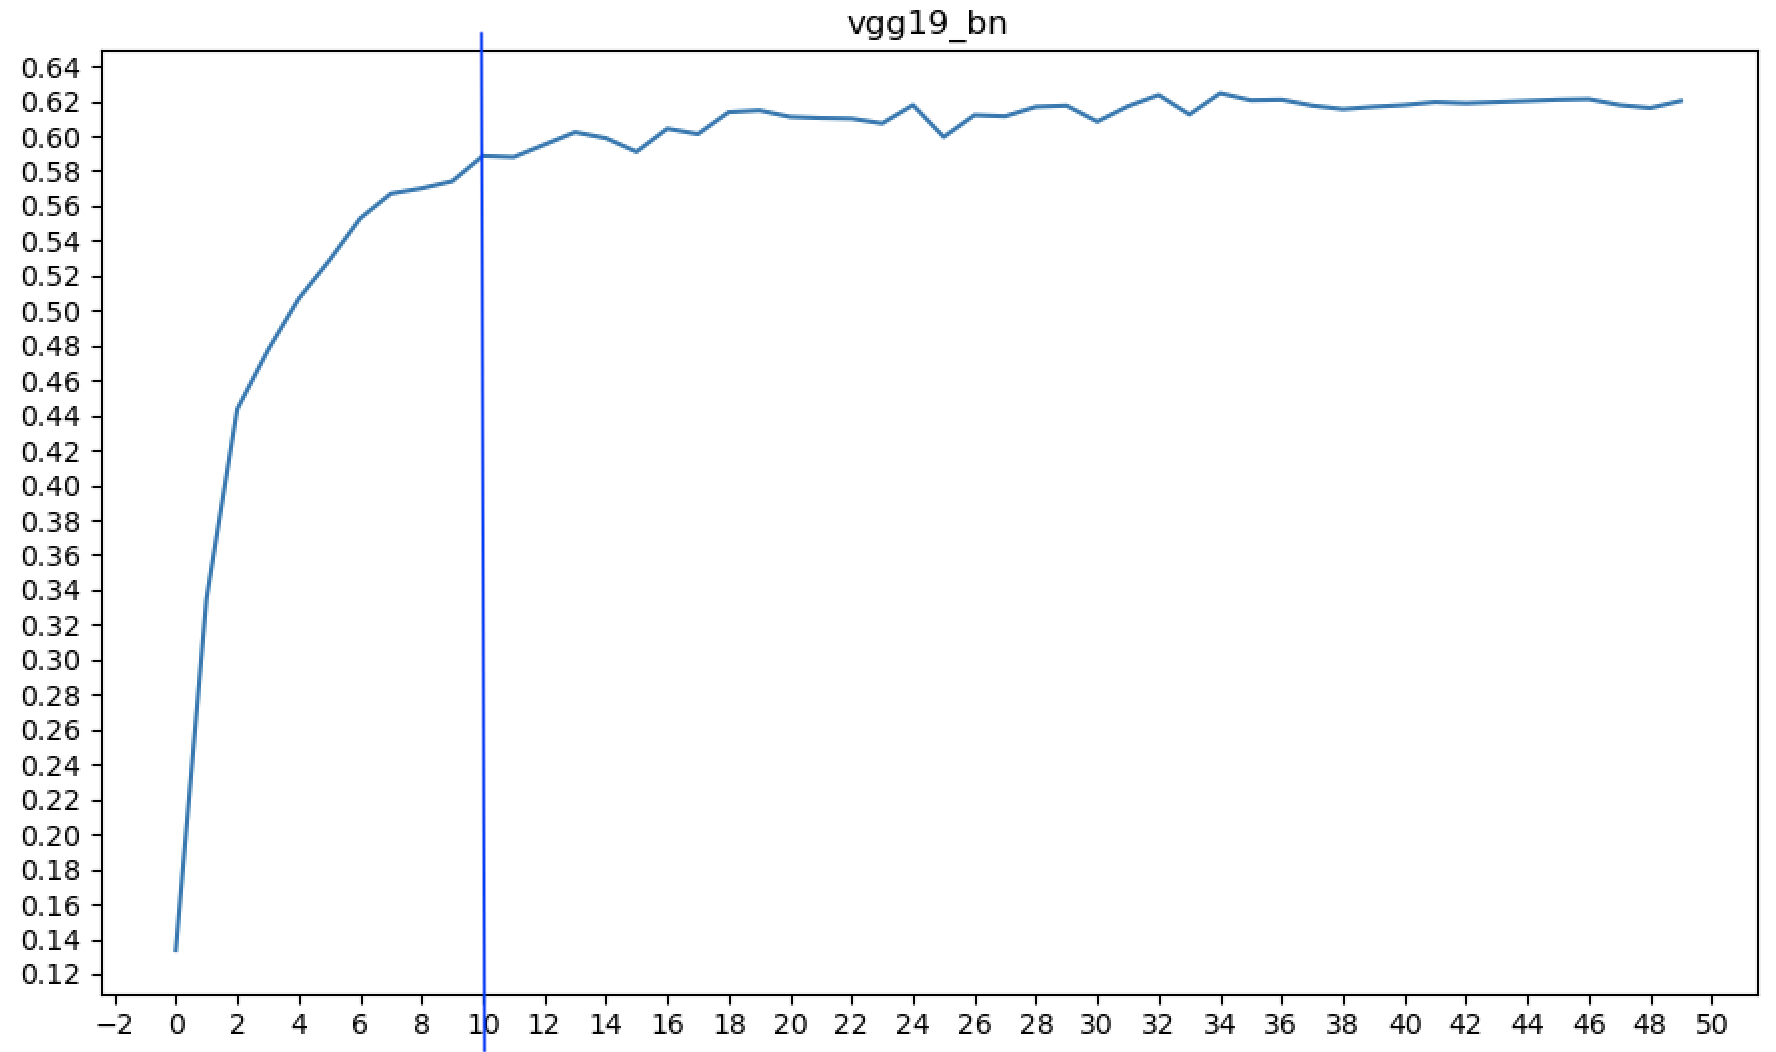
\includegraphics[width = \gws cm]{vgg_19_acc_ep.png}
        \label{fig:vgg_19_acc_ep}
     \end{subfigure}
        \caption{Breaking point of Resnet101 and VGG19}
        \label{fig:sing_acc_ep}
\end{figure}\\



We can further analyse the behaviour of each model for the first 10 epochs by observing Fig. \ref{fig:acc_training_10}. This graph gives us a closer look at how the models have been trained and how the curve looks like. Differently from the previous graph, Resnet152 this time reached a higher accuracy, however it was also the model that took the most time to fully complete the training.\\
On the other hand, from Fig. \ref{fig:acc_training_10}, we can clearly observe  that, if compared with each other for the same training time, shallower networks like Resnet34 or Resnet50 achieved higher accuracy than deeper networks like Resnet152. This is obviously due to the fact that, within the same training time, shallower networks manage to complete more epochs, and therefore complete more training cycles. As a matter of fact, if we were to compare models on an epoch base we will find that deeper networks will achieve better accuracy when given the same number of epochs. \\
If we observe Fig. \ref{fig:com_ti_ac_models} before the 1000 seconds mark, we can see that Resnet18's curve starts to flatten, reaching an accuracy of \textasciitilde 61\%, while the others tend to reach smaller accuracy values. Around the 1000 seconds mark the behaviour of all the models starts to equalise and afterwards the accuracy of deeper networks will increase reaching higher values. As mentioned previously, this is due to the models being able to finish more epochs within the same time frame. In this case, the models reached to finish the training completely, as shown in \ref{fig:com_ti_ac_models}. 
Models from different architectures do not follow this trend. Alexnet, as we already discussed above, does not manage to reach somewhat close to the same accuracy of the other models. VGG16 and VGG19 follow similar trends and both curves overlap multiple times.  Even though VGG19 is considerably bigger than VGG16 (\cite{simonyan2015deep}), they reach very similar accuracy even before the 1000 seconds marks with very similar training time. \\
\begin{figure}[h]
       \centering 
	    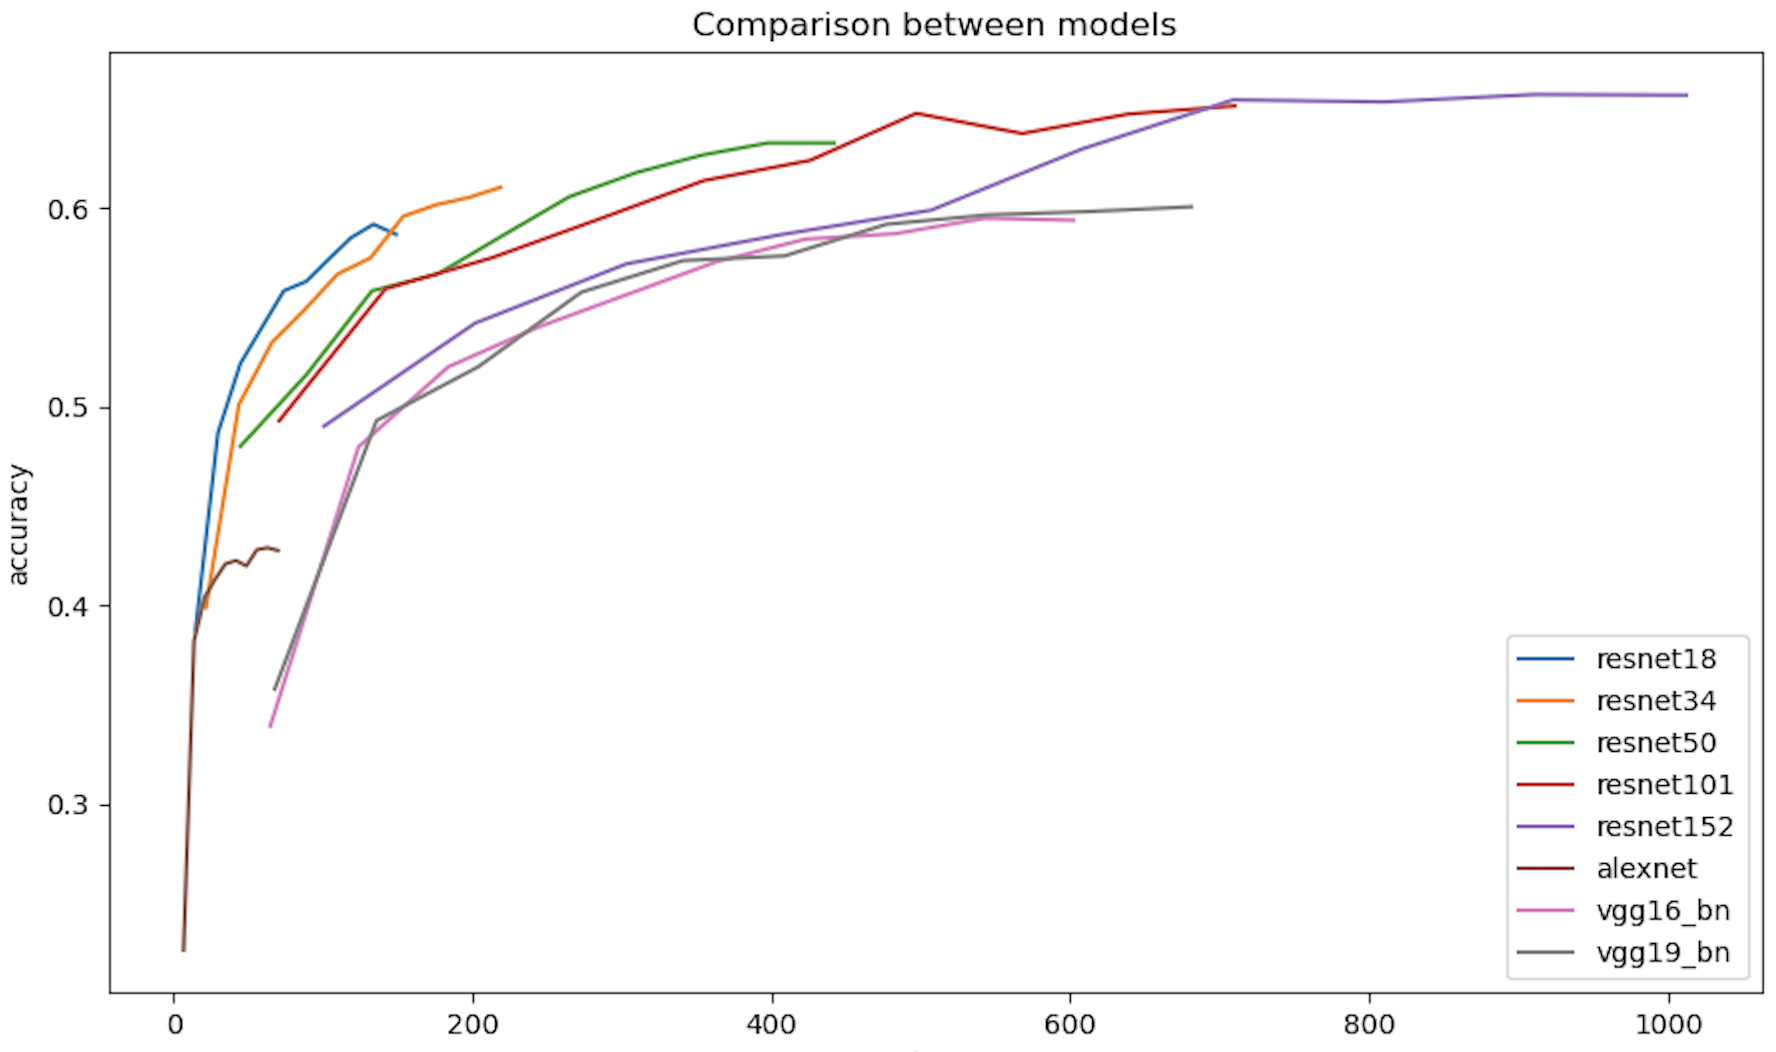
\includegraphics[width = 12 cm]{acc_training_time_10.png}
        \caption[Comparison between training time and accuracy for each model for 10 epochs]{Comparison between training time and accuracy for each model for 10 epochs. The x axis is the training time in seconds, while the y axis is the accuracy achieved}
         \label{fig:acc_training_10}
\end{figure}


\begin{figure}[h]
       \centering 
	    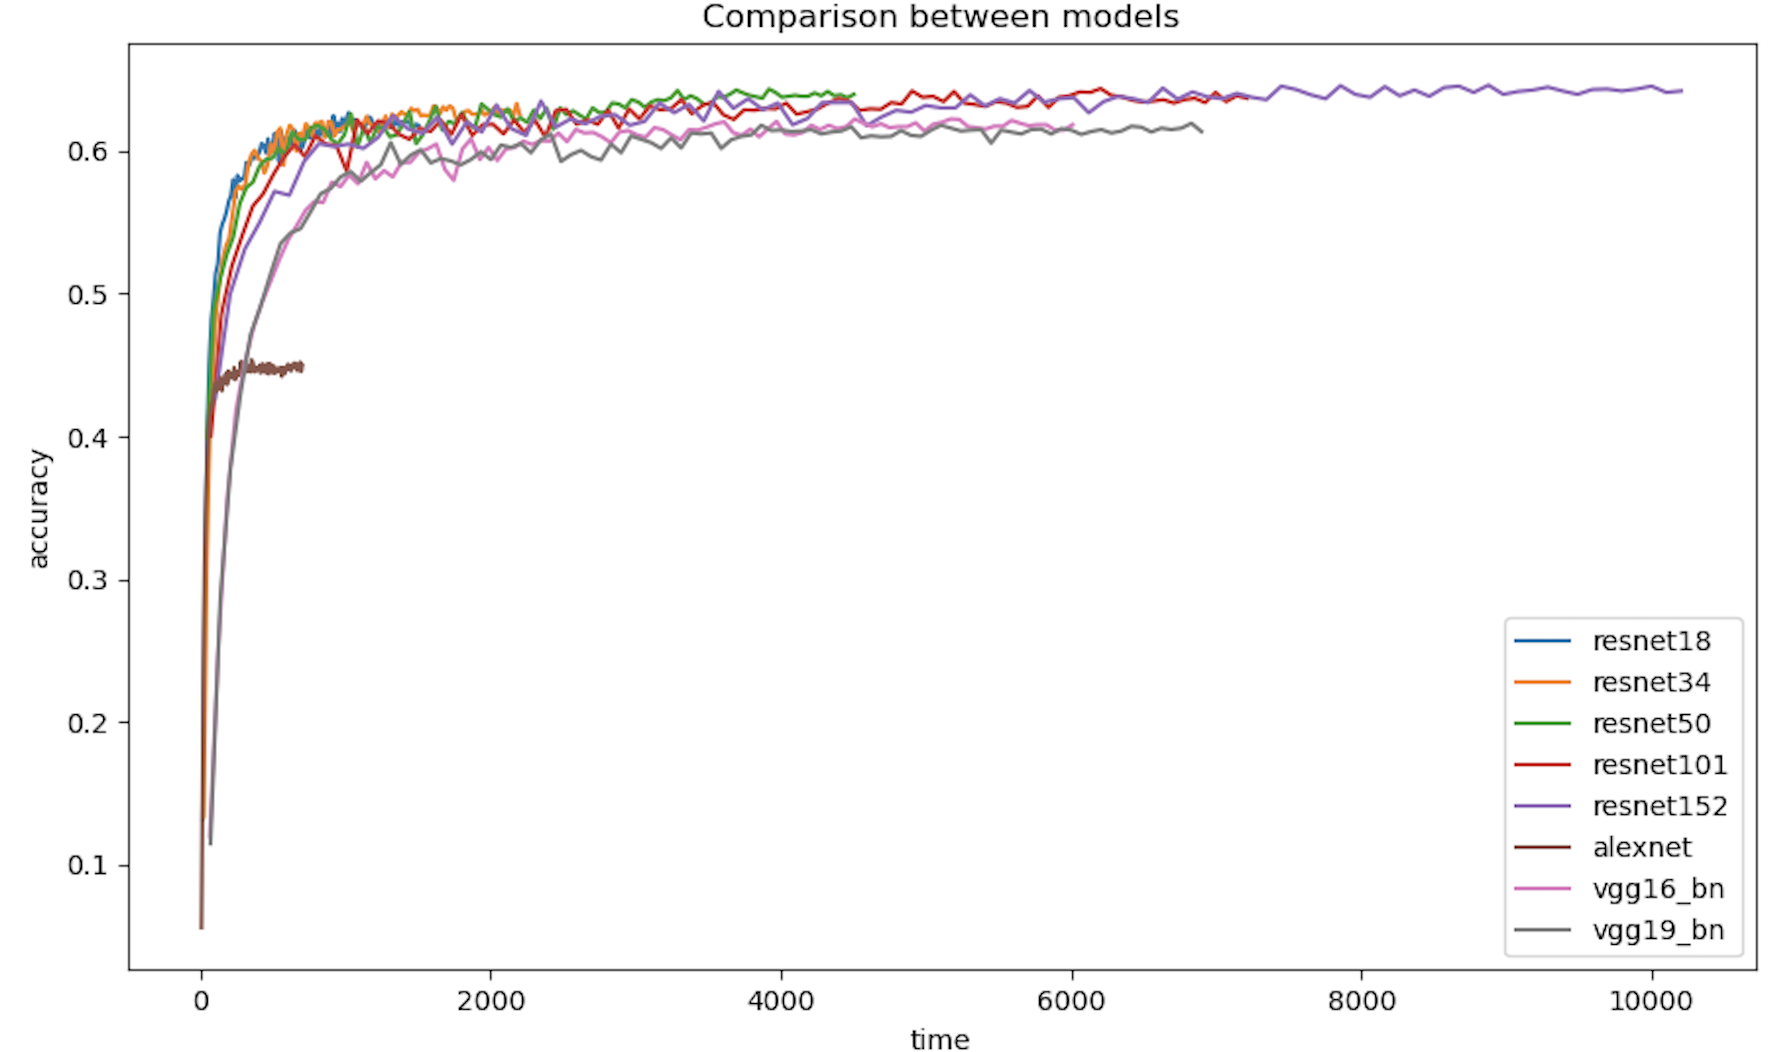
\includegraphics[width = 12 cm]{time_acc_100.png}
        \caption[Comparison between training time and accuracy for each model for 100 epochs]{Comparison between training time and accuracy for each model trained for 100 epochs. The x axis is the training time in seconds, while the y axis is the accuracy achieved}
         \label{fig:time_acc_100}
\end{figure}




This behaviour is further highlighted in Fig. \ref{fig:time_acc_100} which shows the behaviour of the models trained for 100 epochs. We can see that once again around 1000 seconds the curve of every model starts to flatten and the models using the Resnet architectures achieve similar accuracy. The highest accuracy is achieved by Resnet152, which also needed the most training time. Surprisingly, Resnet50 performed better than Resnet101, achieving better accuracy with less training time.
VGG16 and VGG19 performed similarly, displaying overlapping curves, with VGG19 once again requiring more training time. \\
More importantly, however,this graph confirms the results and the hypothesis we made previously. Furthermore, we can use all the data we acquired to calculate the average training time required for each epoch. The results are provided in table \ref{tab:time_f_epoch}.
\begin{table}[h]
\centering
\begin{tabular}{ p{2cm} p{2cm}   }
 Model&Time (s)\\
 \hline
Resnet18&15.01\\
Resnet34&22.0\\
Resnet50&45.02\\
Resnet101&72.11\\
Resnet152&102.02\\
Alexnet&7.01\\
VGG16&60.09\\
VGG19&68.97\\
 \hline
\end{tabular}
\caption{Average time for each epoch}
\label{tab:time_f_epoch}
\end{table}

Comparing the training results we just obtained with the ones obtained for the 'plant\_seedlings\_v2' dataset, we can see that, regardless of the raw values we obtained, the models behaved equivalently in training. \\
Training for 100 epochs also gives us more complete insights regarding the future performance of our models. In other words, we can determine when the model starts to over-fit or under-fit and when to stop the training to avoid future poor performances. \\
\begin{figure}[h]
\begin{subfigure}{0.5\textwidth}
	    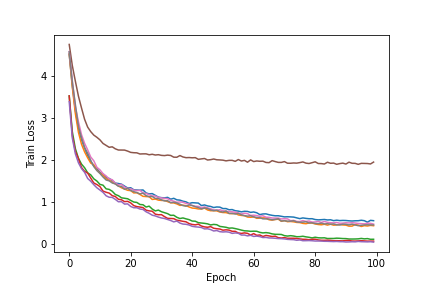
\includegraphics[width = \gws cm]{epoch_train_loss.png}
	    \caption{Training Loss calculated over 100 epochs}
        \label{fig:train_loss}
        
     \end{subfigure} \hfill
     \begin{subfigure}{0.5\textwidth}
	    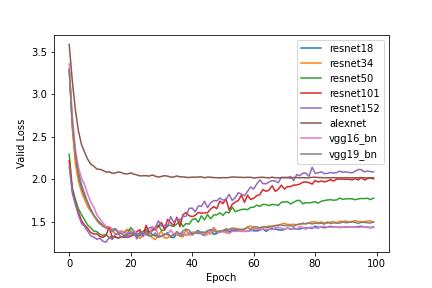
\includegraphics[width = \gws cm]{epoch_valid_loss.png}
	    \caption{Validity Loss calculated over 100 epochs}
         \label{fig:valid_loss}
         
     \end{subfigure}
    
     
     \caption{ Training loss and validity loss of all models calculated over 100 epochs}
        \label{fig:tran_valid_loss}
\end{figure}


As shown in Fig. \ref{fig:train_loss}, the train loss decreases at each epoch for each model. For Alexnet, the curve tends to flatten at around 15 epochs, while for the others it flattens at around 60. Rather than observing the training loss trend alone, however, which does not give us the possibility to comprehend correctly the response of the models, we should compare it to the trend of the validation loss shown in Fig. \ref{fig:valid_loss}. Alexnet remained stable for the duration of the training, with a validation loss comparable to the training loss. The other models, on the other hand, show a rather different behaviour. At around 20 epochs, the validation loss of deeper networks, i.e. Resnet152, Resnet101 and VGG19 starts to increment drastically. For shallower networks of the Resnet architecture, i.e. Resnet18, Resnet34 and Resnet50, and for VGG16 the validation loss decreased for the first 15 epochs and started to increment only after \textasciitilde40.\\
In section n. \ref{sec:of_uf} we defined over-fitting to be a situation in which the validation loss is much larger than training and from Fig. \ref{fig:valid_loss} we can see that, although after various numbers of epochs, most of the networks start to enter this condition as the validation loss increases and it becomes much larger than their training loss. We also discussed some techniques to avoid this, like for e.g. Cross-Validation. For the purpose of this experiment, we only split the dataset 80-20, hence we used no cross-validation or augmentation on the data-set whatsoever. \\
In this analysis, we can observe the first difference with the results obtained in the first experiment. First of all, the training loss decreases rather slowly when compared to Fig. \ref{fig:tran_valid_loss_seeds_res_100} or Fig.  \ref{fig:tran_valid_loss_seeds_res_100_2}. The validation loss, on the other hand, as we already noticed, increased as the training time increased, while for the other experiment it either remained stable, or increased minimally.
To measure inference time, we need to collect a dataset of related pictures, which are not part of the training dataset, to feed to each model. For our tests, we are going to use a data set composed of 200 random pictures. The pictures we are going to use are going to be of different dimensions and different quality in order to see if we can recognize patterns. We can see the results in Fig. \ref{fig:inf_time_epoch_c}, which displays the training time in milliseconds graphed against the accuracy and the number of epoch used to train. From this figure, we can clearly see that the inference time for every model rarely is measured to be more than 230 milliseconds, with the exception of a few outliers, and most of the models for most epochs have an accuracy between 87\% and 92\%. In addition, if we analyse the inference time based on the number of epochs (Fig. \ref{fig:inf_time_epoch}) the models display similar responses.  \\


\begin{figure}[h]
     \begin{subfigure}{0.5\textwidth}
	    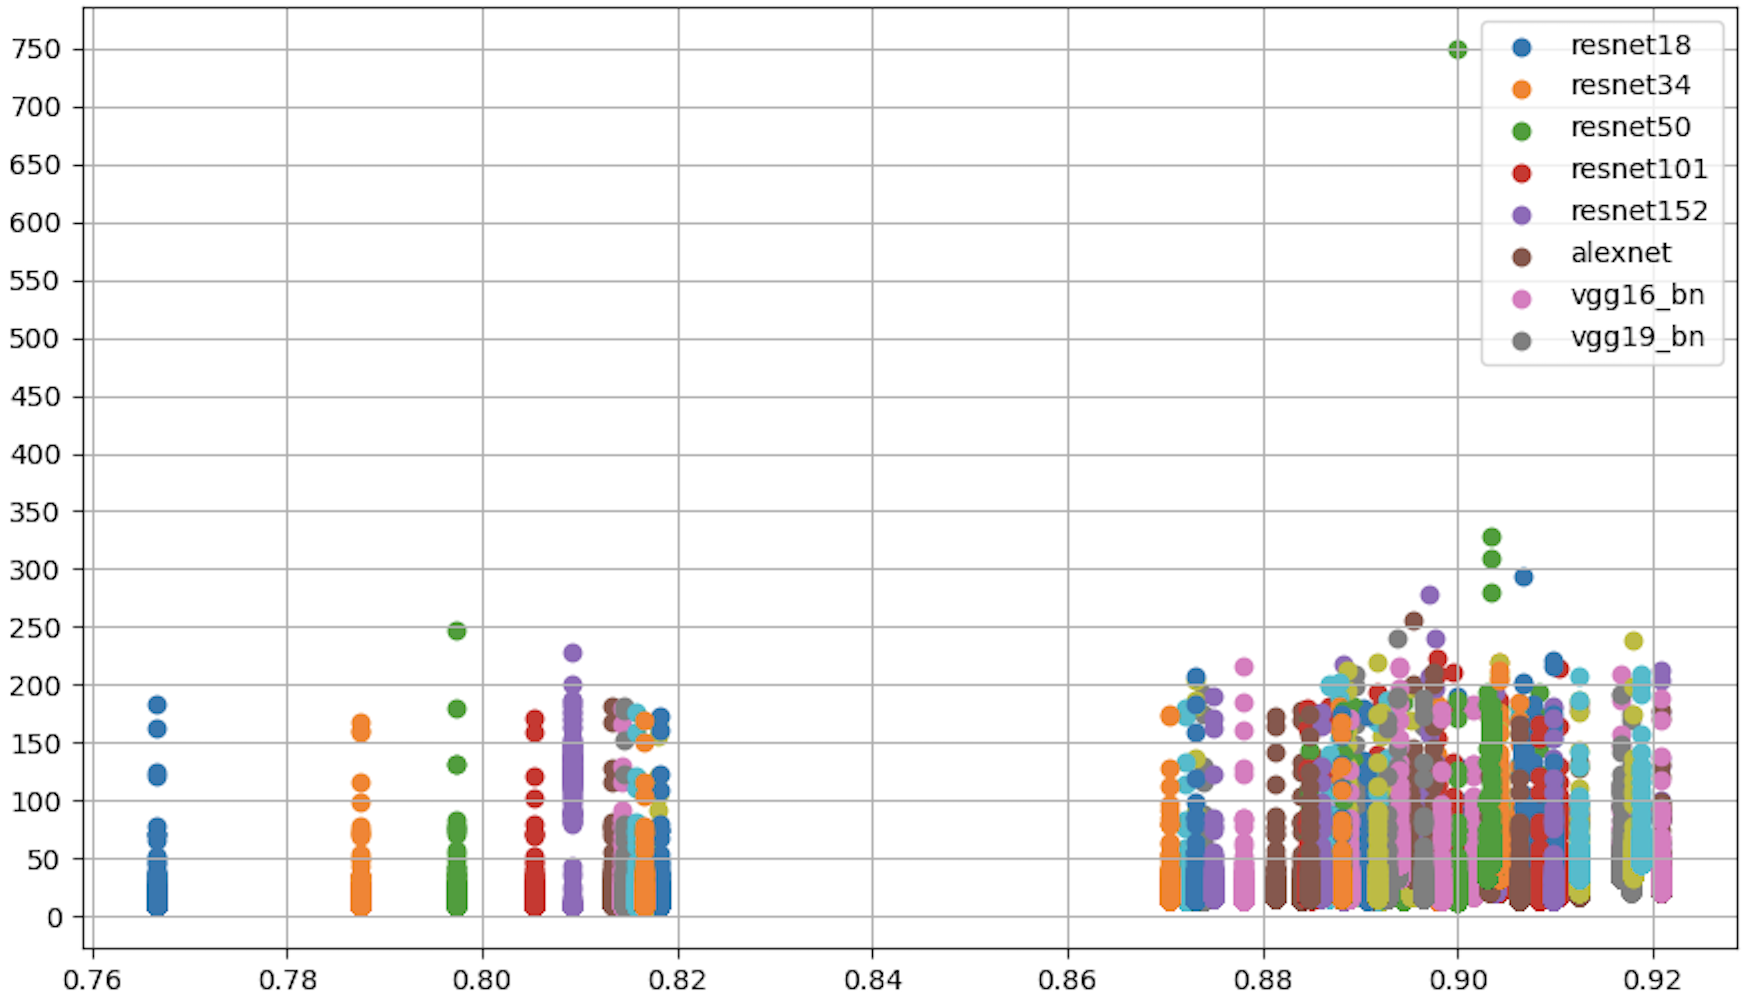
\includegraphics[width = \gws cm]{inf_time_accuracy.png}
	    \caption{}
         \label{fig:inf_time_accuracy}
     \end{subfigure}
     \hfill
     \begin{subfigure}{0.5\textwidth}
	    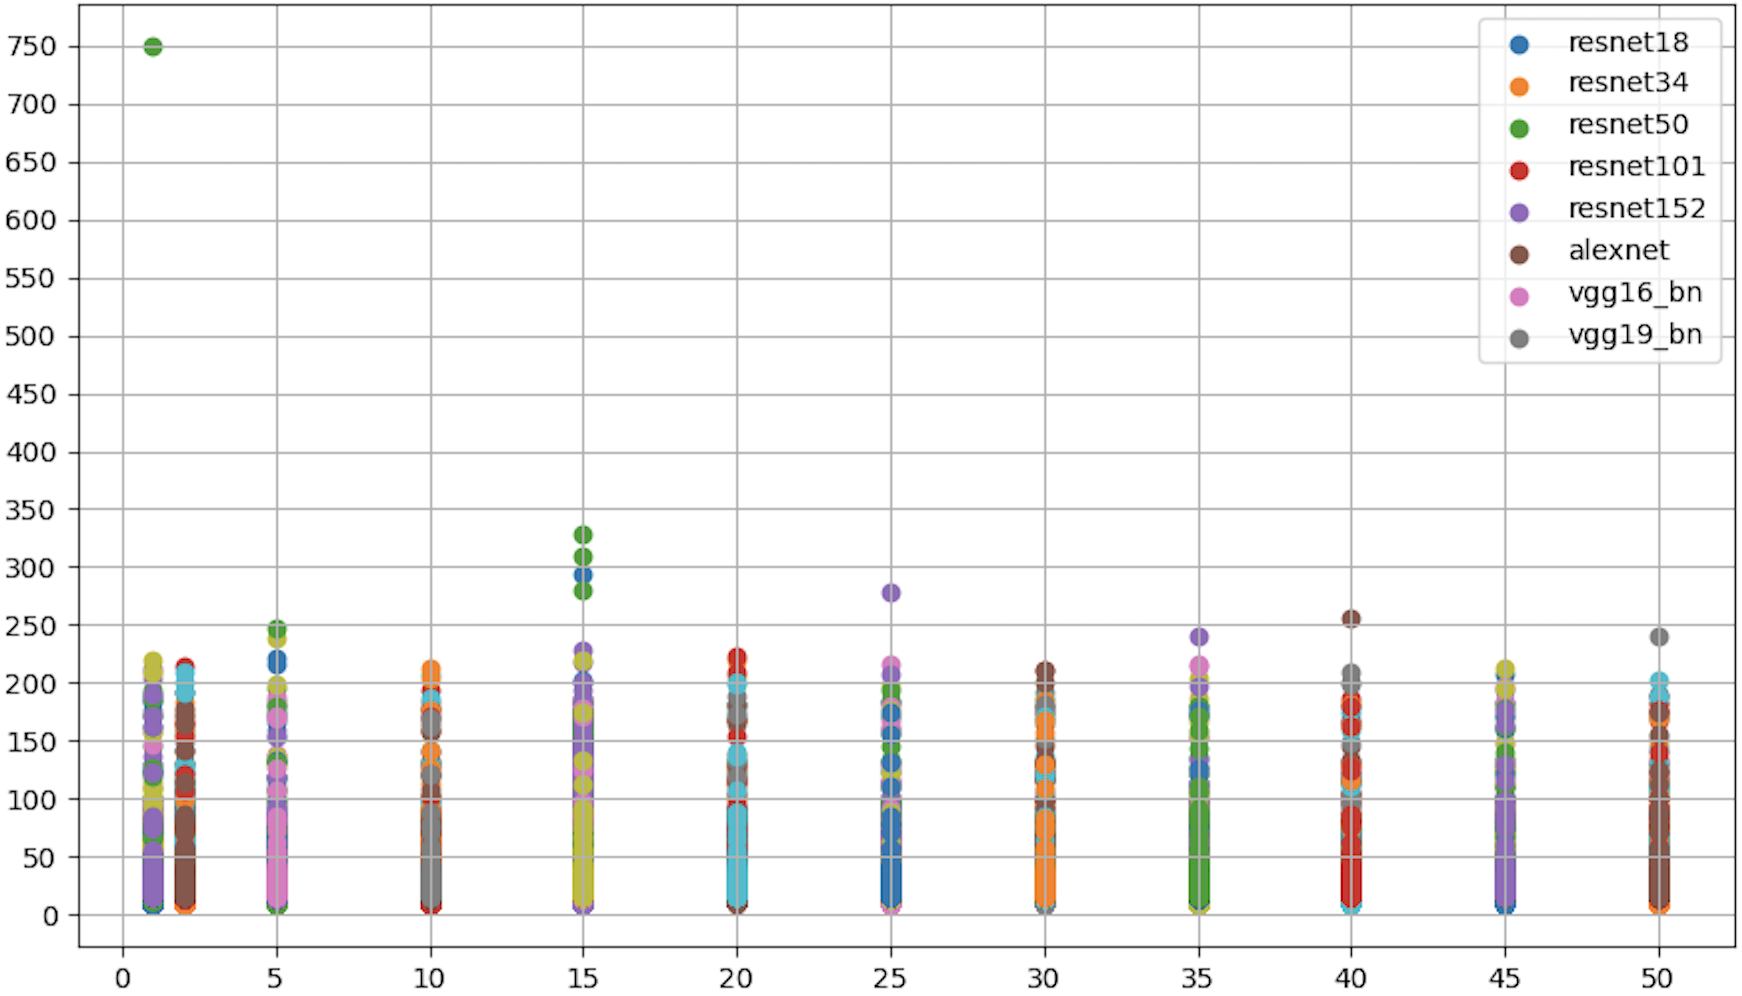
\includegraphics[width = \gws cm]{inf_time_epoch.png}
	    \caption{}
        \label{fig:inf_time_epoch}
     \end{subfigure}\\
     \caption[Inference time measured for each model]{Inference time measured for each model using the 200 pictures dataset discussed previously. The inference time is in milliseconds, while the accuracy for Fig. \ref{fig:inf_time_accuracy}is the percentage of correct predictions.}
        \label{fig:inf_time_epoch_c}
\end{figure}

\begin{figure}[h]
     \begin{subfigure}{0.5\textwidth}
	    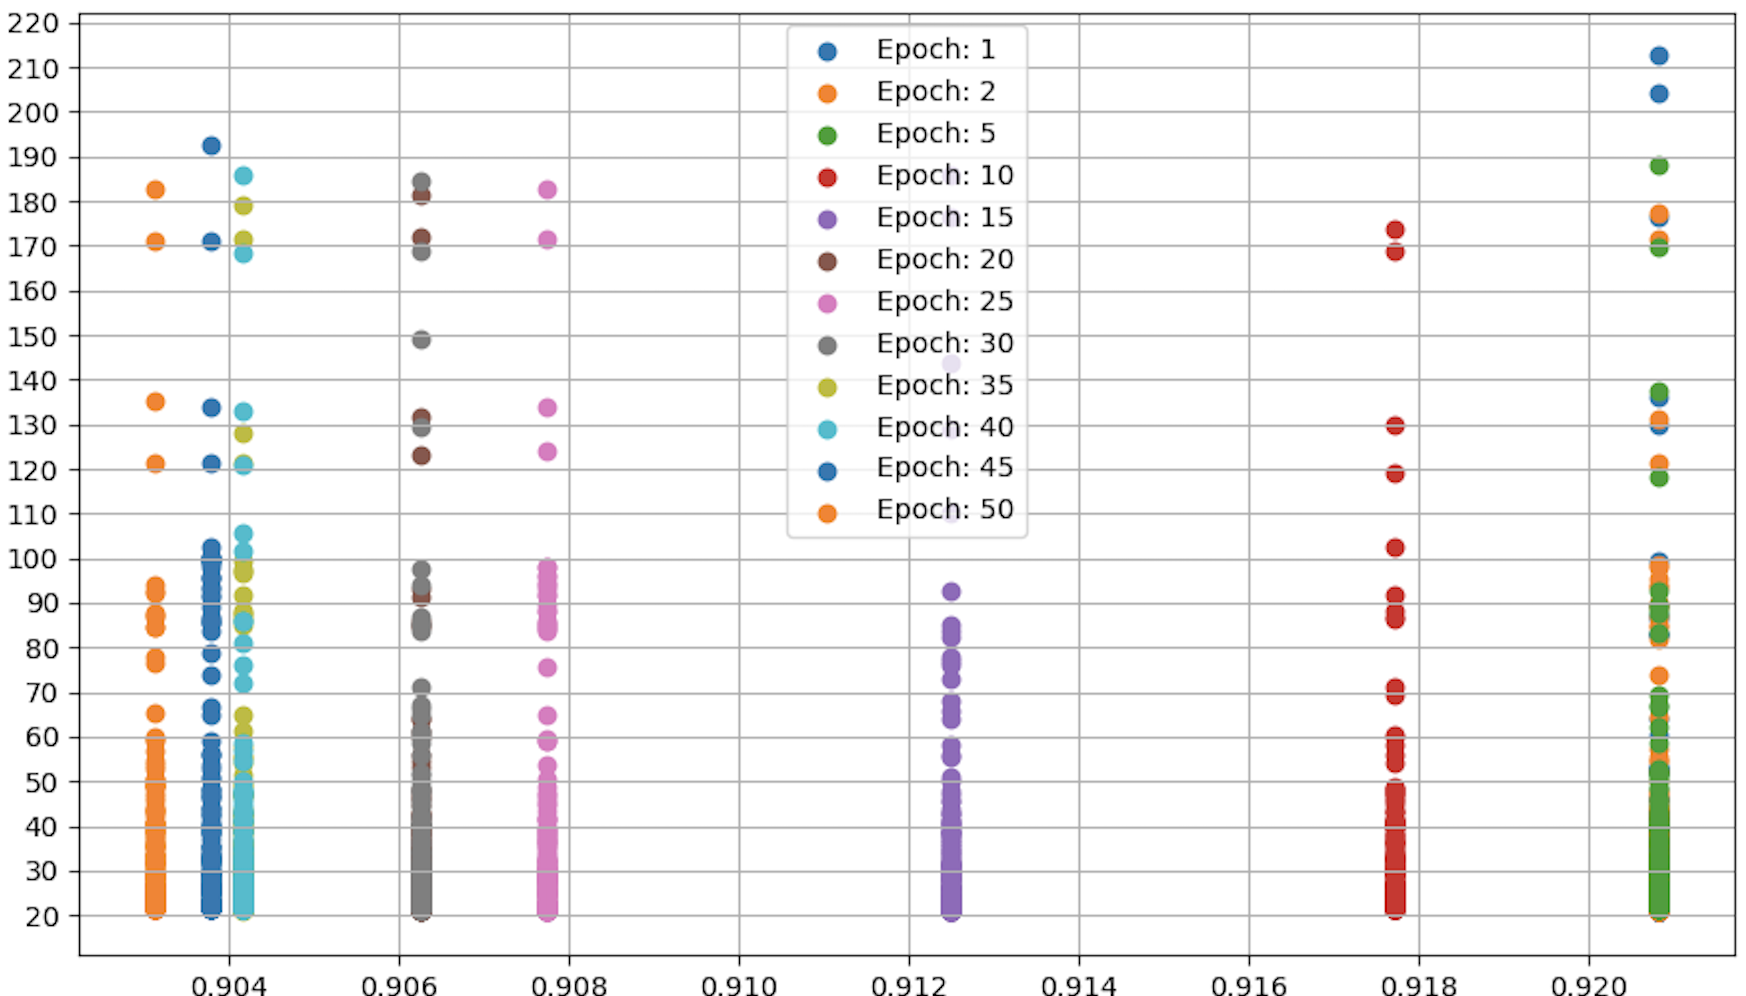
\includegraphics[width = \gws cm]{inf_acc_resnet18.png}
	    \caption{Resnet18}
         \label{fig:inf_acc_resnet18}
         
     \end{subfigure}
     \hfill
     \begin{subfigure}{0.5\textwidth}
	    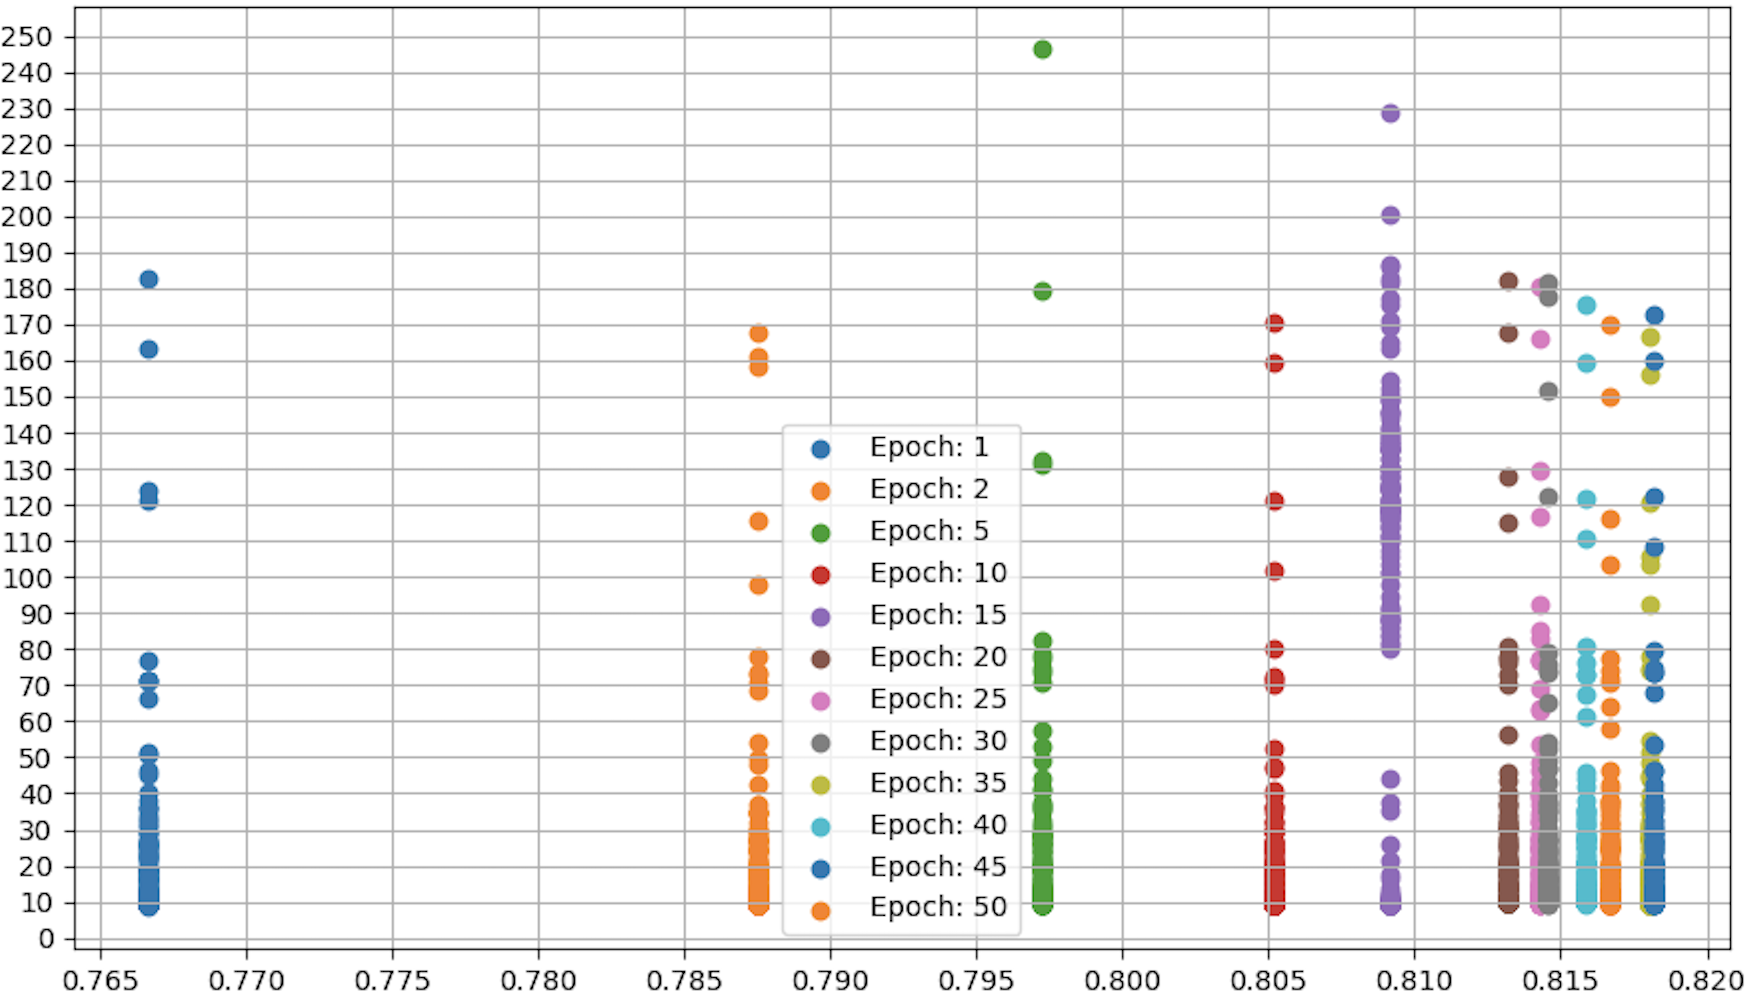
\includegraphics[width = \gws cm]{inf_acc_alexnet.png}
	    \caption{Alexnet}
        \label{fig:inf_acc_alexnet}
        
     \end{subfigure}\\
     \caption{Inference time measured for model Resnet18 and Alexnet}
        \label{fig:inf_acc_c}
\end{figure}
When we compare models individually like in Fig. \ref{fig:inf_acc_c}, other similarities appear. As a matter of fact, when we analyse each model, we can observe that some pictures require considerably more time than others. For example, Fig. \ref{fig:inf_acc_c} shows the measurements obtained by model Resnet18 (\ref{fig:inf_acc_resnet18}) and Alexnet (\ref{fig:inf_acc_alexnet}) and from their response it appears that, at each epoch, there is a constant number of images which takes more time to be processed. \\
We can run the tool once again to identify the 10 images that took more time to be processed at each epoch, in order to analyse them and find elements which can explain such differences. \\
The first property of the image we are going to take a look at is the size of the images. Fig. \ref{fig:size_inference_time_compared} shows the results obtained for each model. 


\begin{figure}[h]
       \centering 
	    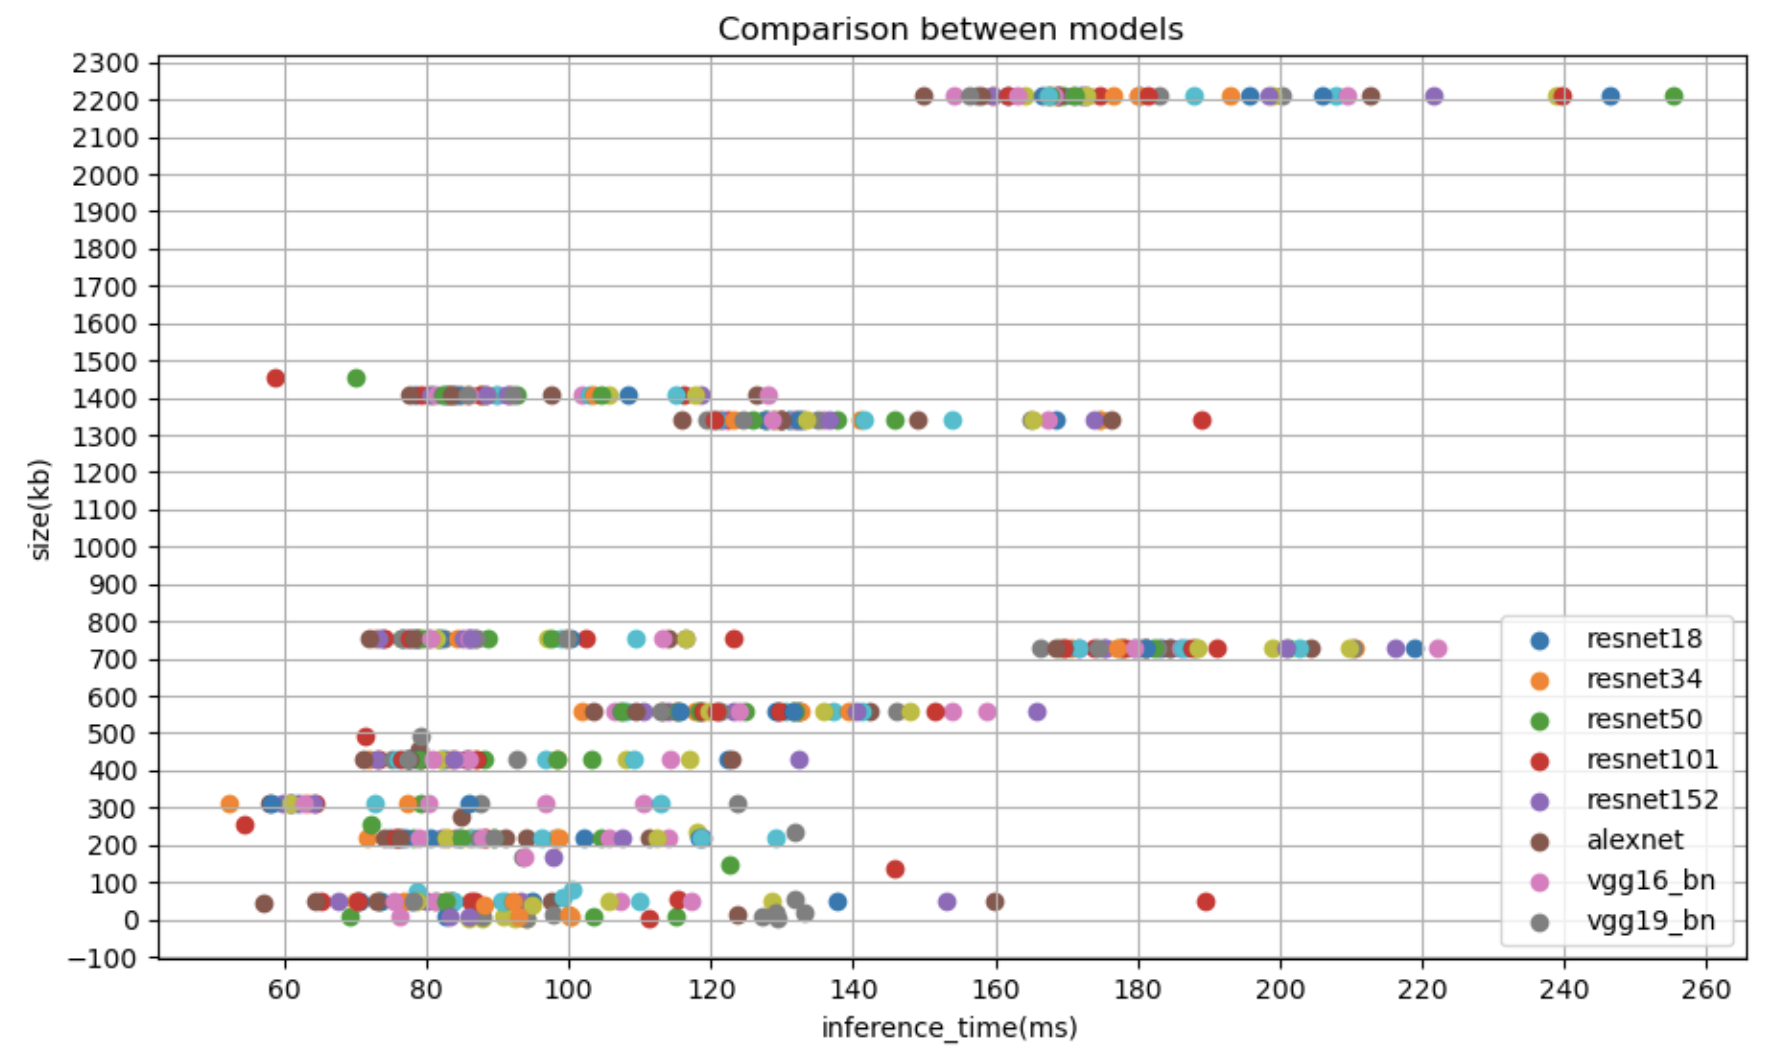
\includegraphics[width = 14 cm]{size_inference_time_compared.png}
        \caption[Size of the images over inference time]{This graph shows the size in kb of the ten slowest images over the time taken to be processed }
         \label{fig:size_inference_time_compared}
\end{figure}



From the graph we are able to spot some rather interesting behaviours. First of all, we would expect that for each epoch the slowest images would be the same. This hypothesis would be confirmed if the graph showed a group of pictures of the same size having different inference times. However, this is only the case for sizes bigger than 500 kbs. As a matter of fact, we are not able to cluster pictures before 500 kb under a certain inference time range as effectively as we can do for heavier pictures. We can conclude from this that regardless of the amount of training, pictures over 500kb are going to be the slowest ones. \\
From a closer investigation of the individual models emerged some differences in the response of the single models. \\
For deeper networks the situation is similar to the discussion we made. As shown in Fig. \ref{fig:sl_f_deep}, for both Resnet152 and VGG16, the response for pictures smaller than 500kb is noisy, although Resnet152 shows a more stable behaviour than VGG16. This implies that for these networks only the response with images over 500kb displays similarities.  
\begin{figure}[h]
     \begin{subfigure}{0.5\textwidth}
	    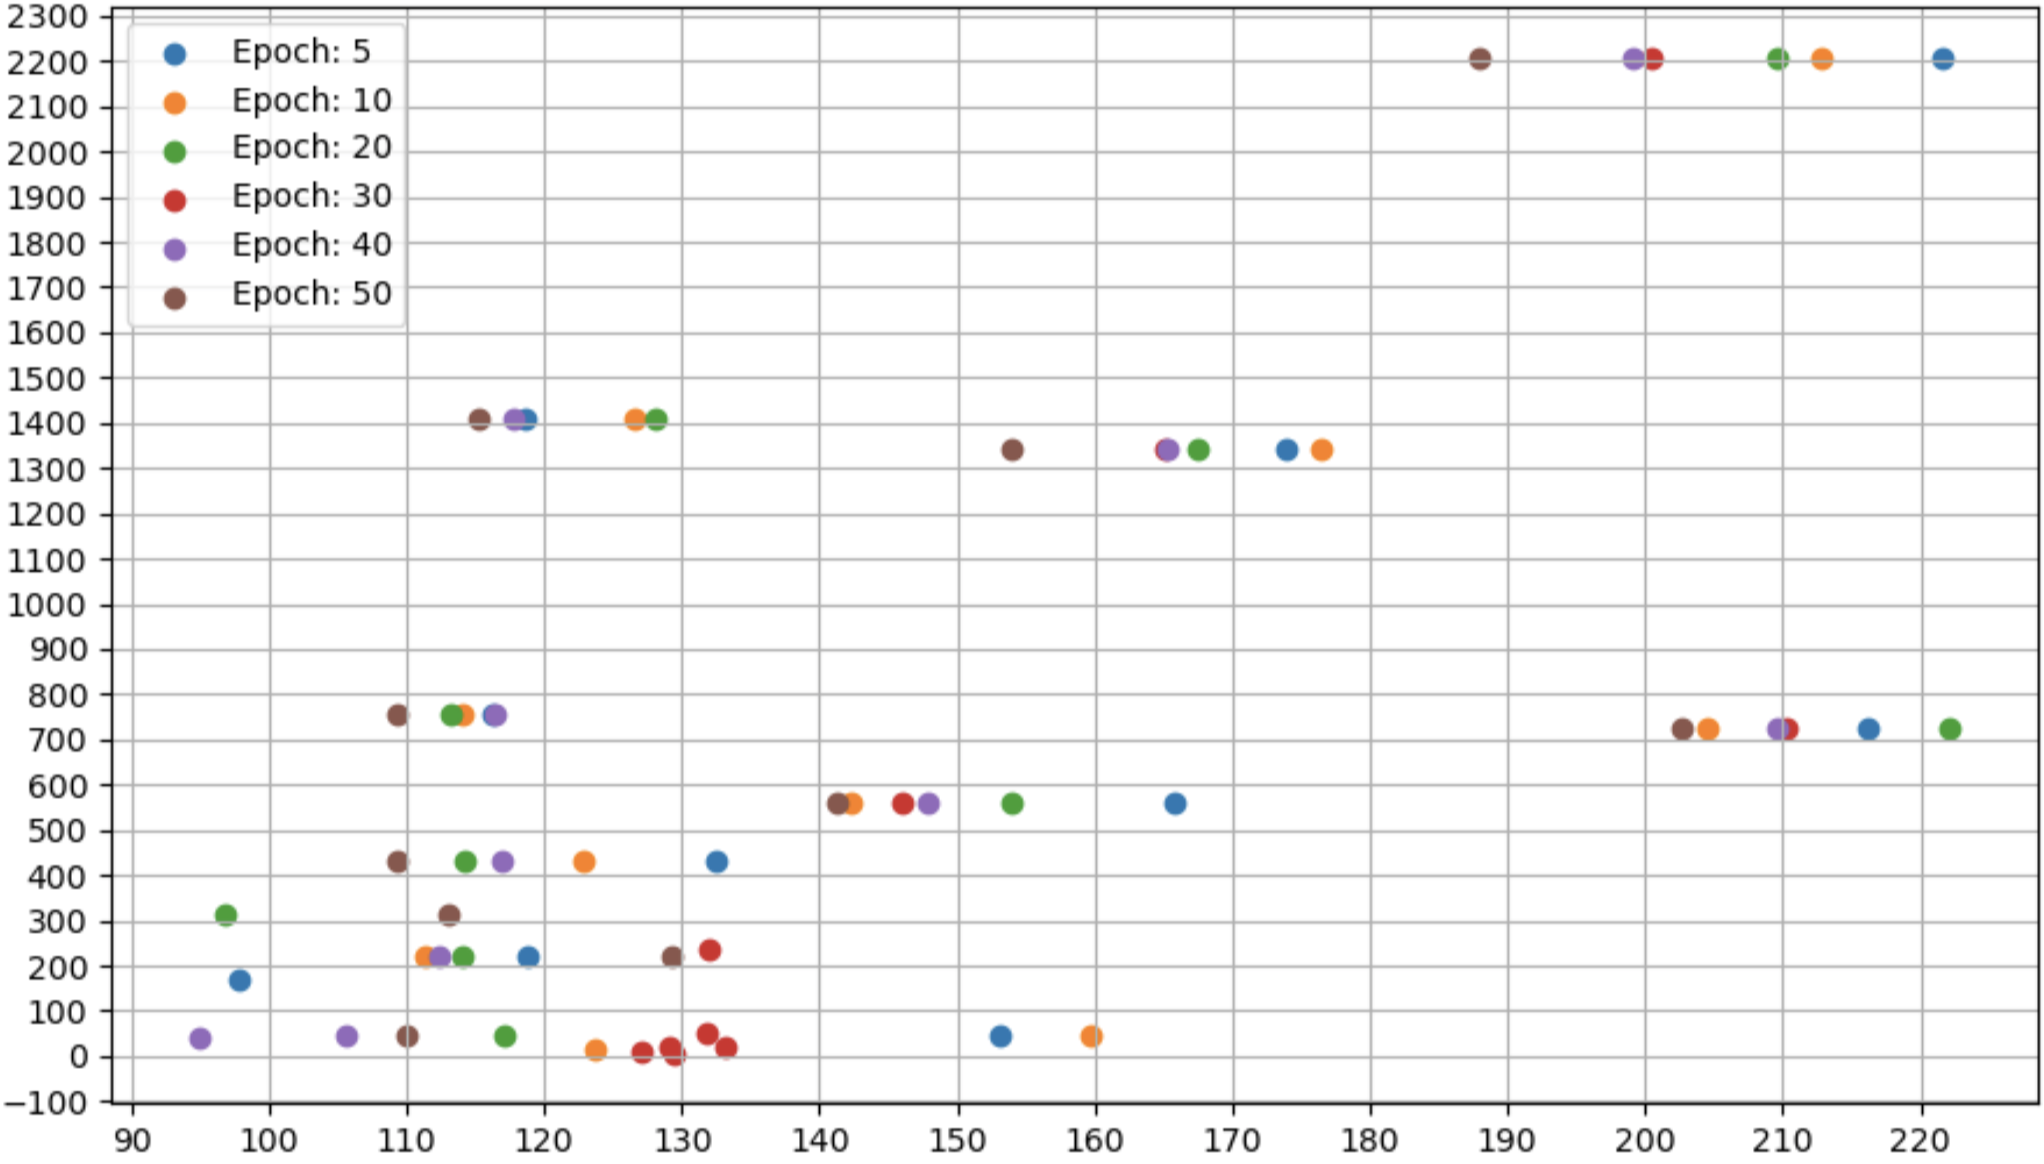
\includegraphics[width = \gws cm]{resnet152_sl_f.png}
	    \caption{Resnet152}
         \label{fig:resnet152_sl_f}
         
     \end{subfigure}
     \hfill
     \begin{subfigure}{0.5\textwidth}
	    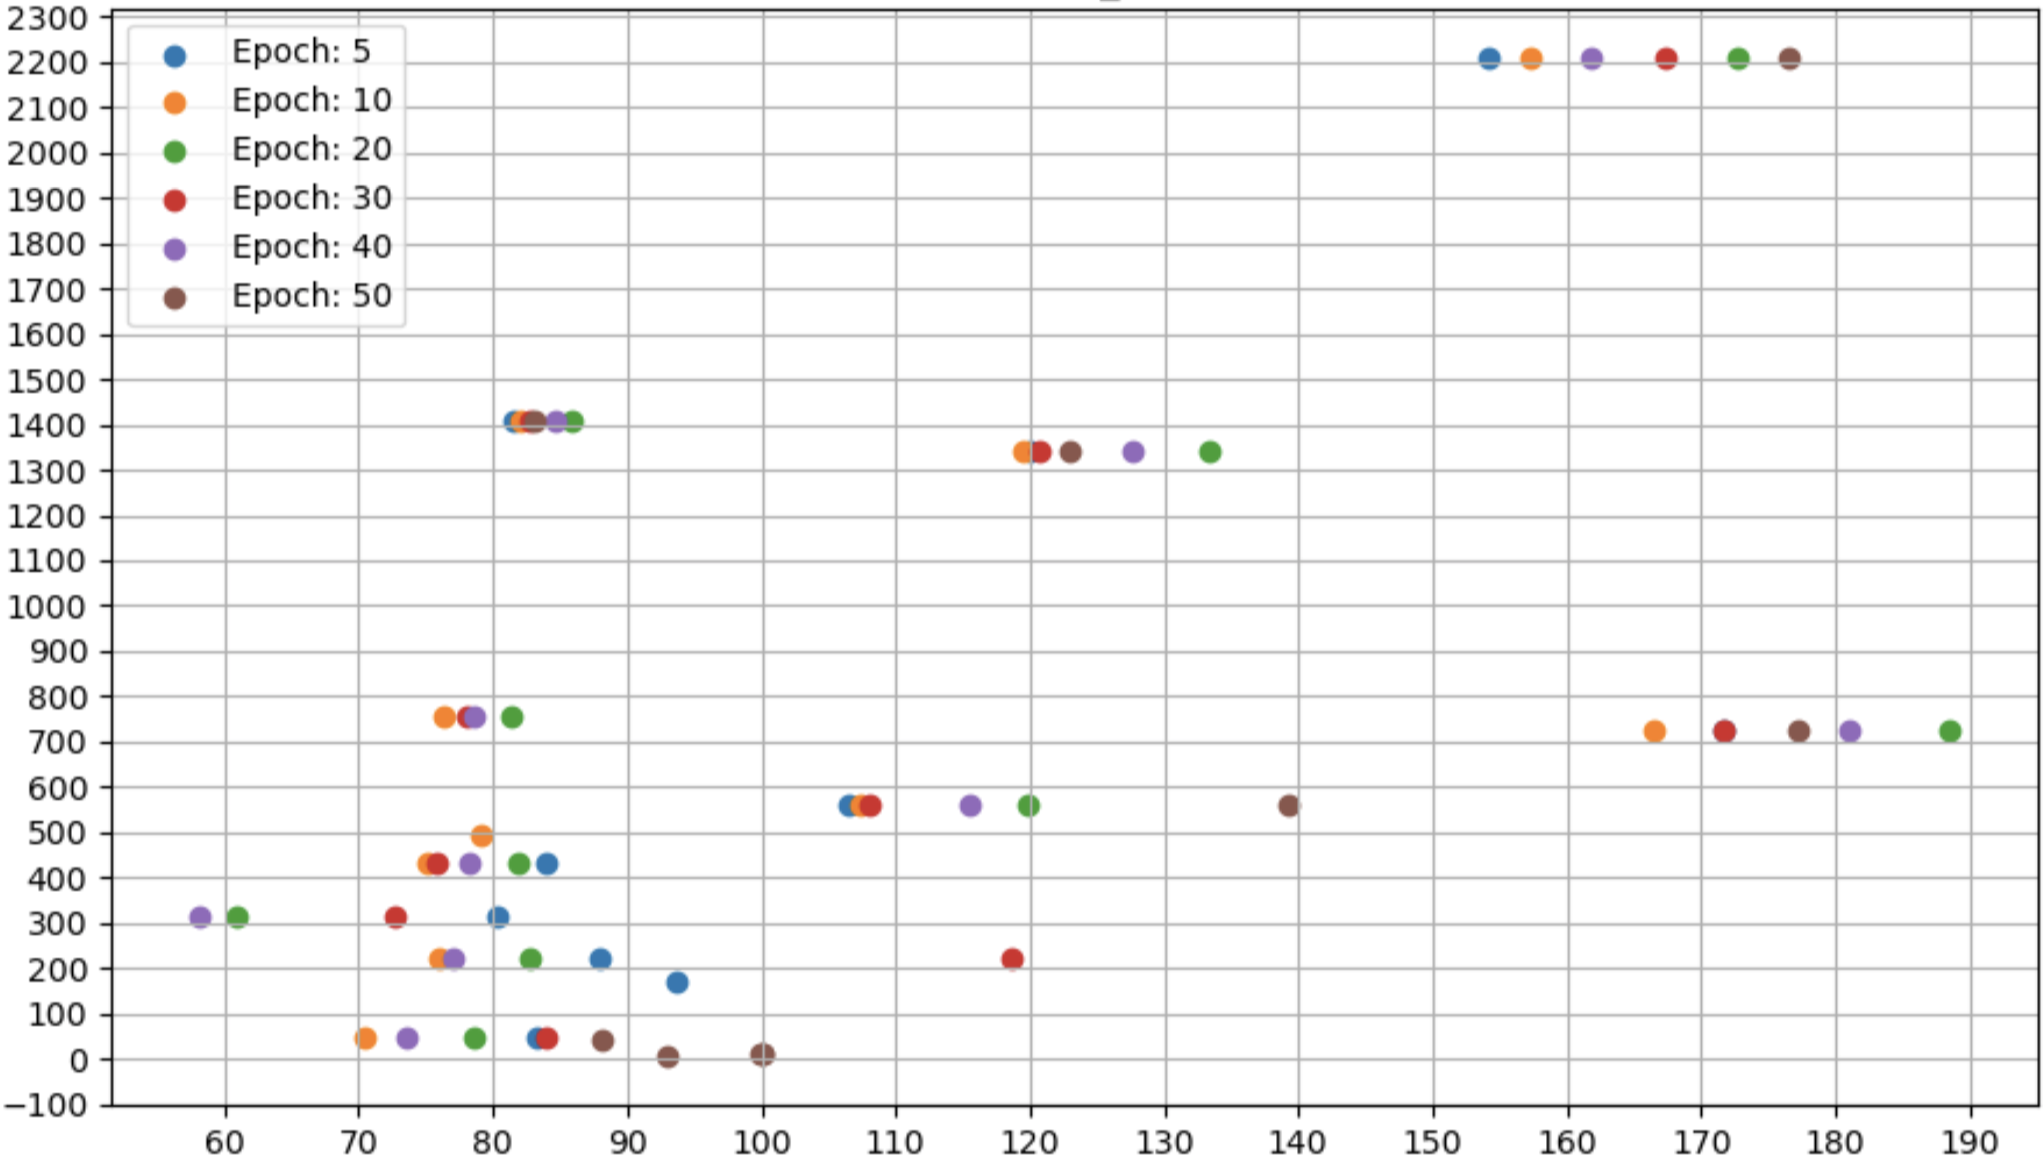
\includegraphics[width = \gws cm]{vgg16_sl_f.png}
	    \caption{VGG16}
        \label{fig:vgg16_sl_f}
        
     \end{subfigure}\\
     \caption{Inference time measured for model Resnet18 and Alexnet}
        \label{fig:sl_f_deep}
\end{figure}

For shallower networks, however, the situation is slightly more different. Fig. \ref{fig:sl_f_shallow} shows the slowest images identified in the models Resnet18 (Fig. \ref{fig:resnet18_sl_f}) and Alexnet (Fig. \ref{fig:alexnet_sl_f}). Differently from what we concluded before, these models show a much more precise response for images smaller than 500 kb. We are in fact able to cluster the images by size, with the exception of very few outliers. In addition, we can also point out which number of epochs would yield faster predictions for the slowest images. For Resnet18, we can observe that the model trained with 40 epochs is among the fastest for most sizes (with very few exceptions). For Alexnet, on the other hand, the fastest model is the one trained for only 10 epochs. This conclusion, however, does not take into account the accuracy that those models achieved. Using Fig. \ref{fig:inf_acc_resnet18} we can see that the same models, i.e. Resnet18 trained with 10 epochs, achieved one of the lowest accuracy rate overall (\textasciitilde90\%) and from Fig. \ref{fig:inf_acc_alexnet} we can extrapolate a similar conclusion for Alexnet trained with 10 epochs. (\textasciitilde80\%). \\
The best trade off between fast inference time and accuracy is achieved when both models have been trained with 50 epochs, however, in case of Resnet18, as we discussed before, this is also the number of epochs in which the validation loss is bigger than the training loss, hence we found ourselves in a situation of slight over-fitting. \\
\begin{figure}[h]
     \begin{subfigure}{0.5\textwidth}
	    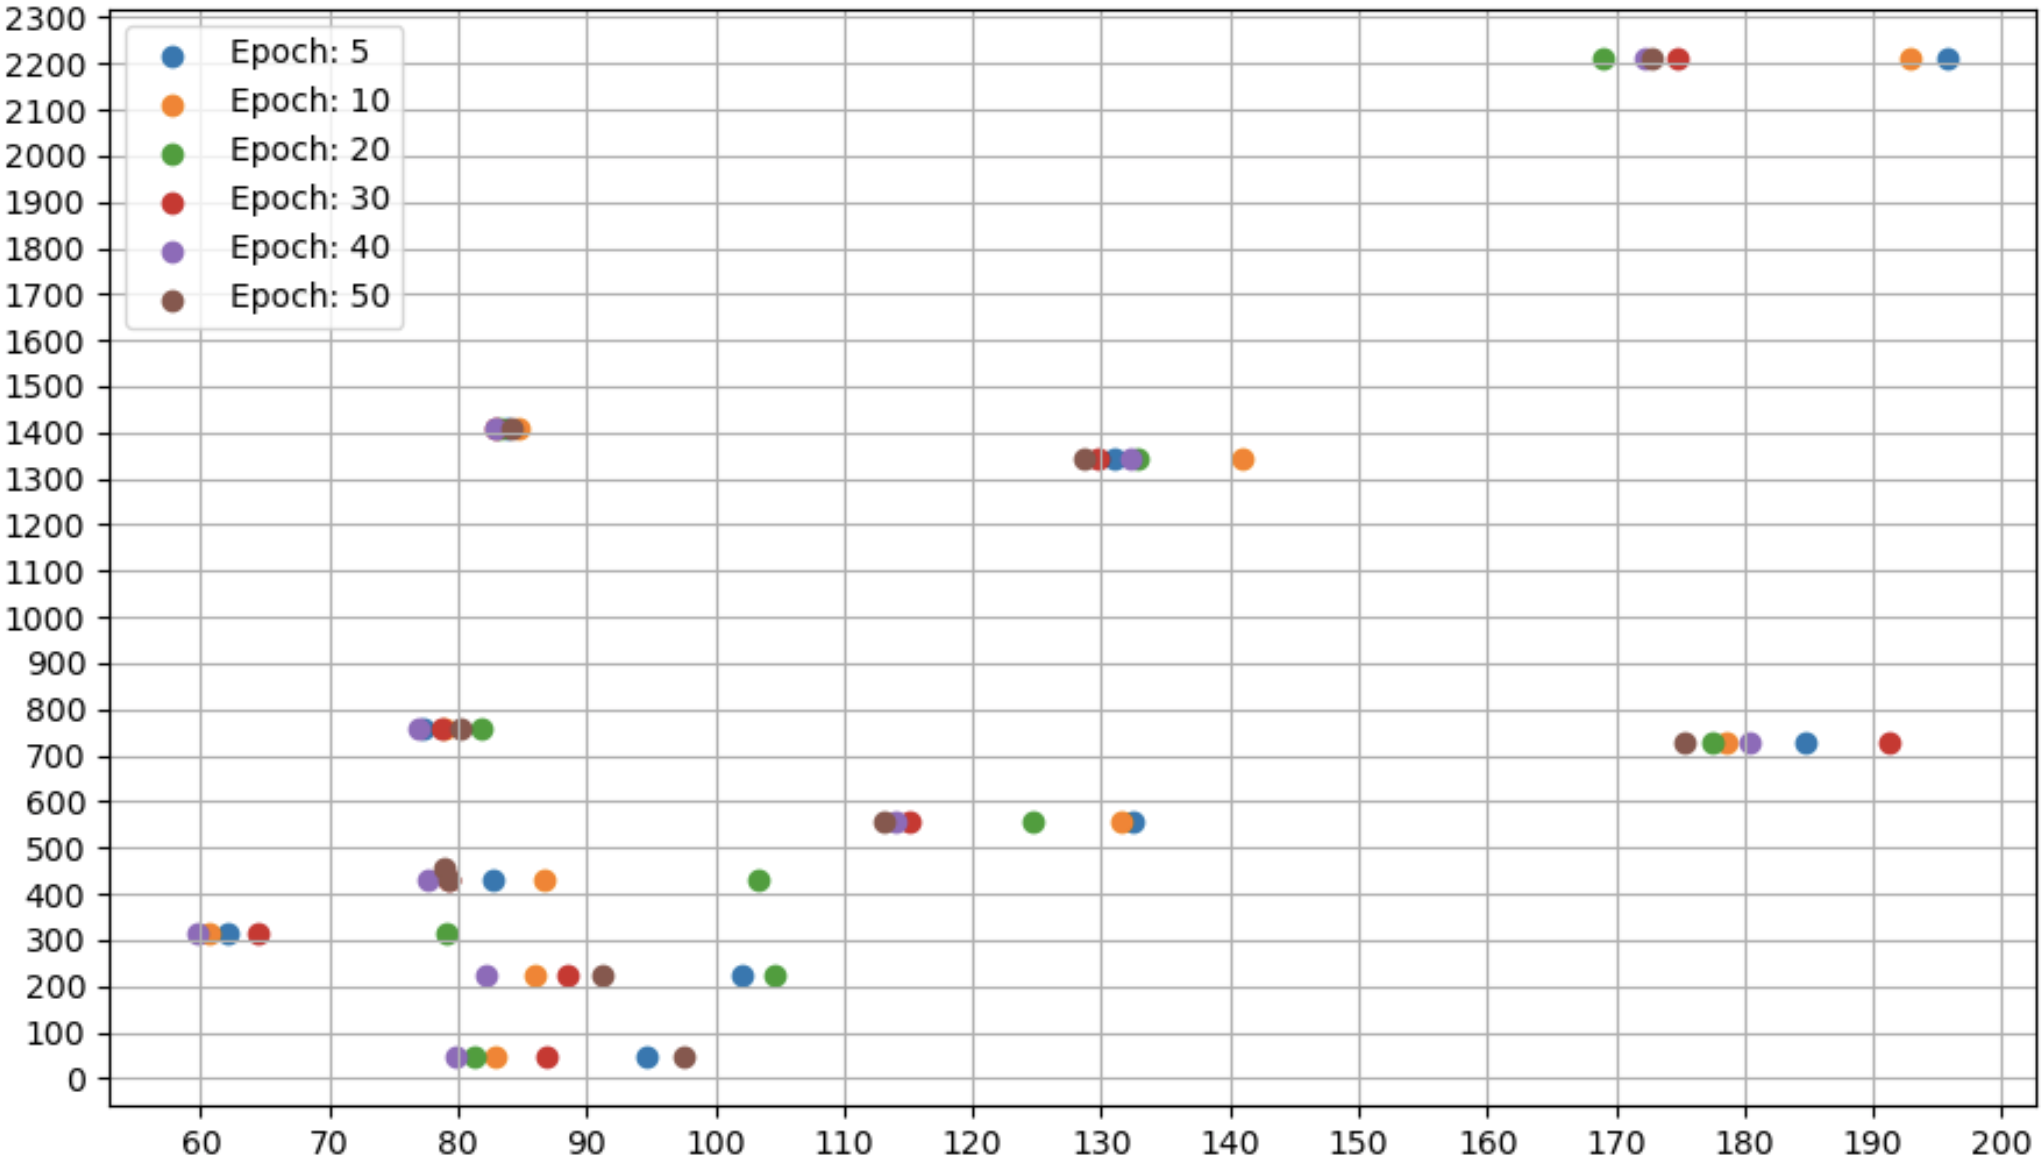
\includegraphics[width = \gws cm]{resnet18_sl_f.png}
	    \caption{Resnet18}
         \label{fig:resnet18_sl_f}
         
     \end{subfigure}
     \hfill
     \begin{subfigure}{0.5\textwidth}
	    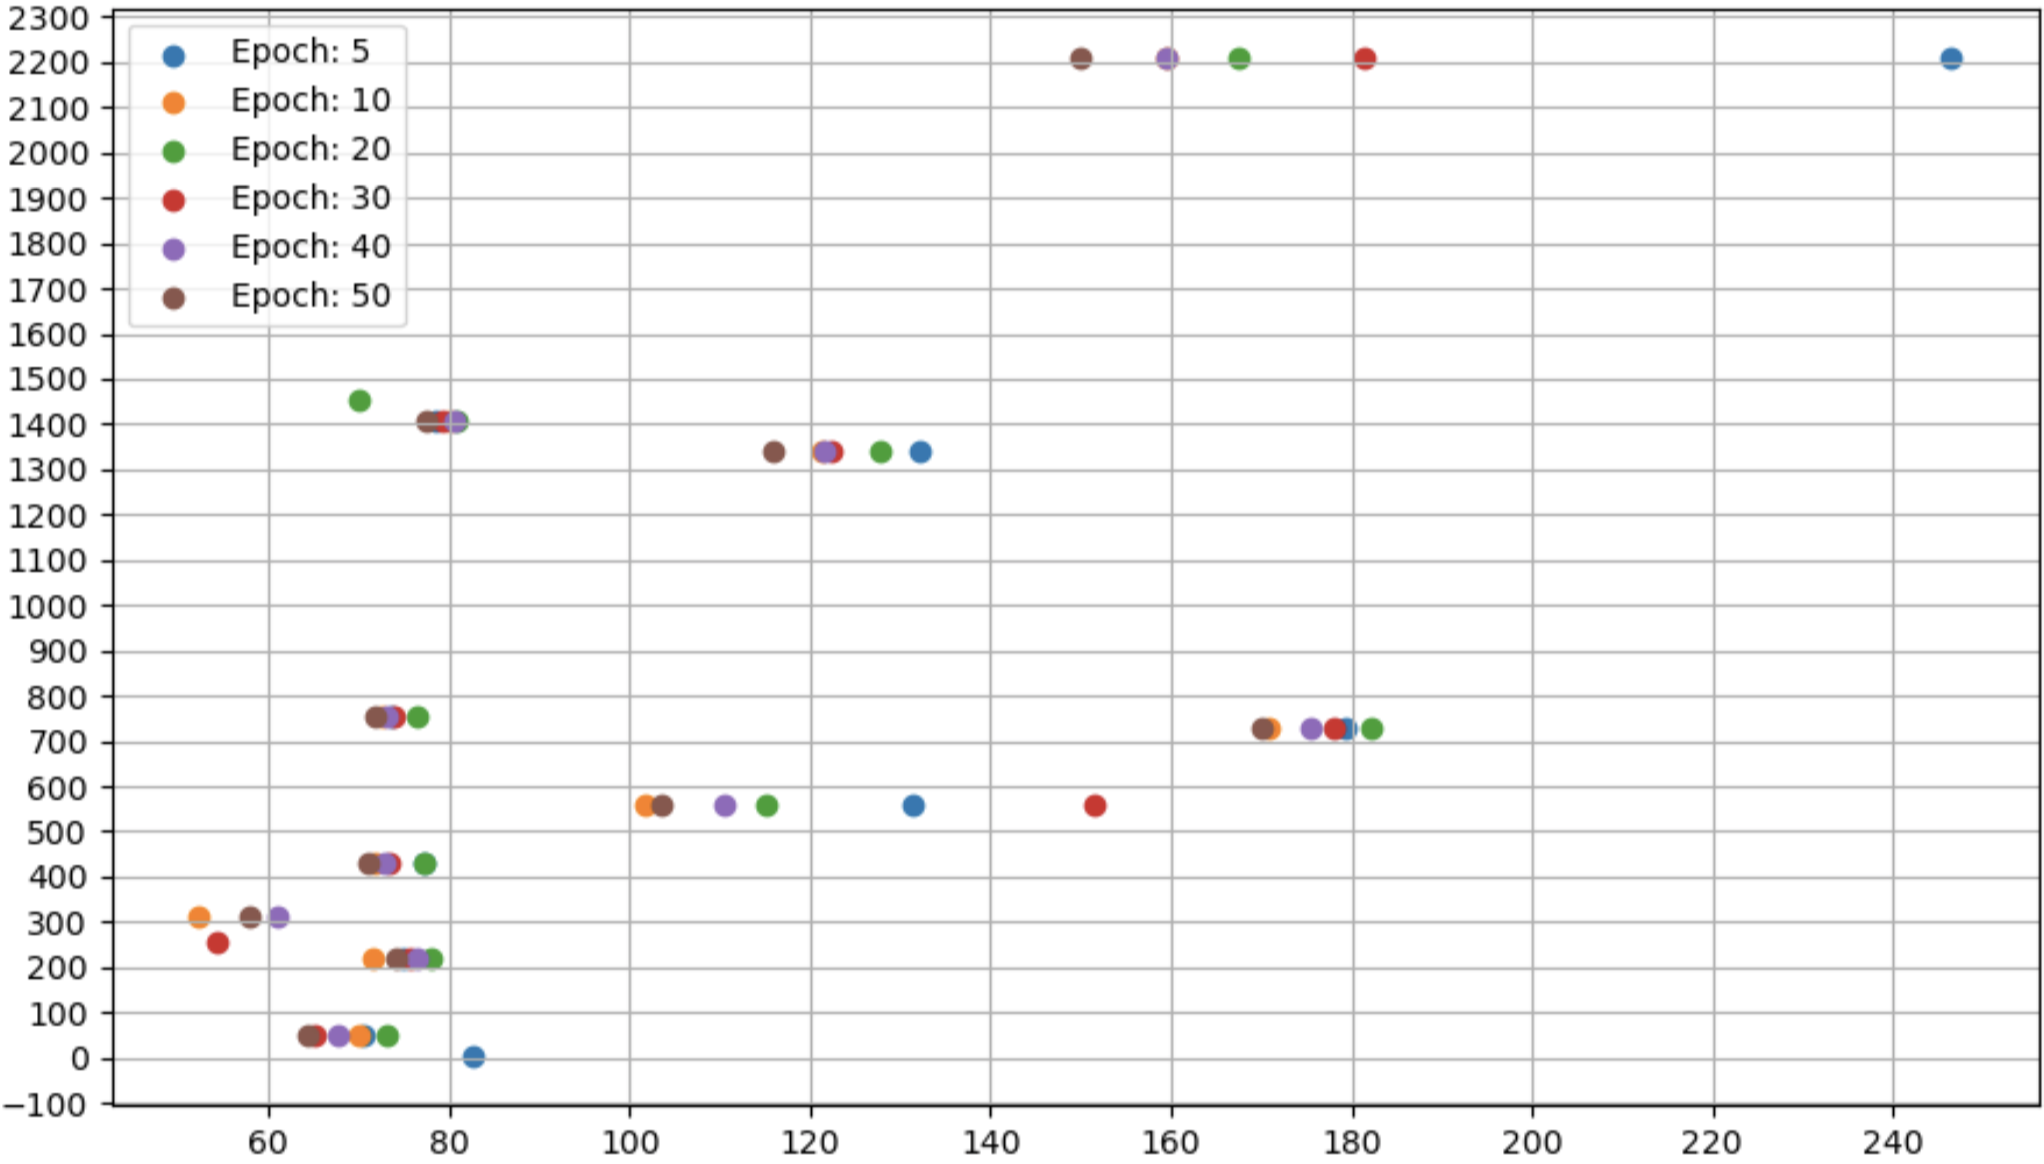
\includegraphics[width = \gws cm]{alexnet_sl_f.png}
	    \caption{Alexnet}
        \label{fig:alexnet_sl_f}
        
     \end{subfigure}\\
     \caption{Inference time measured for model Resnet18 and Alexnet}
        \label{fig:sl_f_shallow}
\end{figure}


Regardless of which number of epochs is better for this specific case, the purpose of our exploration is to identify correlation between certain characteristics. From these graphs we are able to find a correlation and to reason about it, in order to tailor future applications. \\
In a real world implementation, if it is known that images with a certain size are going to be among the slowest is useful because it will influence the decision of which hardware to mount on the devices sent to the fields. Additionally, knowing that images with a size of 700 kb are going to take from 200 to 220ms to be classified, will, naturally, help model the time behaviour of these devices and give information to verify that they will not miss any deadline. Furthermore, if we are able to reason about the trade-off between inference time and accuracy, we would also be able to choose a suitable model for different requirements. For example, in applications in which the system needs to respect a hard-deadline, inference time plays a more important role than overall accuracy. By being able to predict both inference time and accuracy from other characteristics, we can find a trade-off which will allow us to respect any hard-deadline. 


A closer look to the list of slowest images reveals that there are common pictures amongst all models (Fig. \ref{fig:slowest_files_all}). Using the tool we can investigate if those pictures present similarities that may explain why this is the case. The information collected from the pictures are shown in table 
\ref{tab:pictures_info}.

\begin{table}[htbp]
\centering
\begin{tabular}{ p{2cm} p{4cm}  p{2cm}  p{2cm}  }
 Picture n.& Dimensions(x,y) & DPI(x,y)&size(kb) \\
 \hline
1&(3888, 2187)&N/A& 727\\
2&(3018, 2585)&(300,300)&2209\\
3&(3000, 2019)&(300,300)&1341\\
4&(2003, 2003)&N/A&558\\
5&(1373, 1012)&(72,72)&1409\\
6&(2048, 1551)&(300, 300)&221\\
 \hline
\end{tabular}
\caption{Information collected from the slowest pictures}
\label{tab:pictures_info}
\end{table}

As already demonstrated by Fig. \ref{fig:size_inference_time_compared}, each of the five pictures has a size bigger than 500kb, i.e. they are amongst the heaviest pictures on the dataset. Furthermore, they are also amongst the pictures having the highest dimensions. Even though not available for all the pictures, table \ref{tab:pictures_info} also shows that the pictures have high DPI, which implies that these pictures have very high quality. \\
Following the calculations we delineated in section \ref{sec:ben_inf}, we can hypothesise that images with higher dimensions are more slowly processed by the models. This is due to the fact that each architecture presents pooling layers, which according to equation \ref{eq:Pl_FLOPS}, is directly proportional to the dimensions of the images. If we compare Fig. \ref{fig:size_inference_time_compared} and table \ref{tab:pictures_info}, we can also spot a quite interesting relation.
For example, if we analyse picture number 6, we can see that it has a size of 221 kb and dimensions of $2048 \times 1551$ pixels. According to our hypothesis, we would expect it to be slower than pictures having lower dimensions. However, picture 5, with dimension $1373 \times 1012$ pixels, is being processed more slowly or equally by every model at every epoch. We can therefore confute the hypothesis that we just made and conclude that the inference time is influenced not only by the dimension of the images, but also by other characteristics of the images. Studying and analysing these characteristics can produce further results that have not been considered in this paper. % lazy Luca




